\documentclass[11pt]{article}
\usepackage[utf8]{inputenc}
\usepackage{geometry}
\usepackage{graphicx}
\usepackage{hyperref}
\usepackage{amsmath}
\usepackage{listings}
\usepackage{xcolor}
\usepackage{float}
\usepackage{subcaption}
\usepackage{algorithm}
\usepackage{algpseudocode}
\usepackage{booktabs} % For prettier tables
\usepackage{siunitx}
\usepackage{amssymb}
\usepackage{subcaption}
\usepackage{booktabs}
\usepackage{tikz}  % For better table lines
% Set page margins
\geometry{a4paper, margin=1in}

% Set up code listing style
\lstset{
    basicstyle=\ttfamily,
    commentstyle=\color{gray},
    keywordstyle=\color{blue},
    stringstyle=\color{red},
    showstringspaces=false,
    captionpos=b
}

% \title{Discovering Symbolic Models from Deep Learning
% with Inductive Biases: Reproduction Report}
% \author{Vishal Jain}
% \date{\today}
\begin{document}
\begin{titlepage}
    \centering
    \vspace*{1cm}
    
    
\includegraphics[width=0.5\textwidth]{figs/logo.png} % Change this line to the path where you save the Cambridge logo image
    
    \vspace{1.5cm}
    
    {\Large\bfseries Discovering Symbolic Models from Deep Learning with Inductive Biases - Reproduction Report\par}
    
    \vspace{2cm}
    
    {\Large Vishal Jain \par}
    
    \vspace{1cm}
    
    {\large Department of Physics \par}
    \vspace{1cm}
    {\large MPhil in Data Intensive Science \par}
    \vspace{1cm}
    {\large Supervisor: Dr Miles Cranmer \par}
    
    \vfill
    A dissertation presented for the degree of\\
    Master of Philosophy
    
    \vspace{0.8cm}
    
    \Large University of Cambridge\\
    \today % Or specify a date
    
\end{titlepage}
Word Count: 6220
\tableofcontents
\newpage
\section{Introduction}
% Introduce what this report is tackling: reproducing subset of results from Cranmer et al.

% Why is the problem important: Motivate why even bother to develop a framework that approximates nns with symbolic models.

% How are we going to do it: High level overview of the approach taken in the report.

% Background: 
% New concepts - symbollic regression, graph neural networks. Inductive biases.



% What is the report about
The aim of this report is to reproduce the key results of the paper \textit{Discovering Symbolic Models from Deep Learning with Inductive Biases} by \textit{Cranmer et al.} \cite{cranmer2020discoveringsymbolicmodelsdeep}. The main contributions of the paper are two fold - first the presentation of a systematic framework whereby inductive biases can be employed to distill low dimensional symbolic approximations of learned neural networks. The second is showing its successful application of the framework in 3 contexts: rediscovering force laws, rediscovering Hamiltonians and discovering a new equation for a nontrivial cosmology problem.
% What are subset are we exploring 
The scope of this report is limited to the reproducibility of the experiments relating to the rediscovery of force laws. However, in doing so, the wider contribution of the framework is validated.
% Why.
\subsection{Motivation}
Why would it be desirable to approximate a high dimensional neural network with a low dimensional symbolic model? The answer lies in the scientific method itself and the unreasonable effectiveness of mathematics in the natural sciences. When using neural networks as a tool for science, the lack of interpretability is a major drawback. Science is not just about making predictions, but also about understanding the underlying mechanisms that govern the phenomena being studied. Neural networks are famously known to be black boxes, with the decision-making process being opaque to the user. If they are to be used for science, there needs to be some distillation of what the network has learned in a form that is interpretable to humans.  Symbolic models are a natural choice for this task, as they provide a compact and interpretable representation of the underlying mechanisms due to their low dimensionality. Further, they are likely to generalise better to out of distribution data than the neural network itself, indeed this was the shown to be the case in the findings presented by the original paper. Choosing to describe the world in terms of closed form low dimensional mathematical equations seems to be a very good inductive bias.


\subsection{Inductive Biases}
Understanding effective inductive biases is crucial in machine learning. Inductive biases are the priors placed on the space of solutions by a given set of assumptions made explicitly and implicitly when using any modelling process. To demonstrate the importance of selecting appropriate inductive biases, consider an experiment involving a neural network and symbolic regression. In this experiment, depicted in Figure \ref{fig:nn_vs_sym_sin}, a neural network with a single layer of 100 ReLU activations is trained on data sampled from a sinusoidal function. Due to its architecture, the network employs linear piece-wise approximations, which may fit the training data adequately but will extrapolate linearly, leading to poor generalization on out-of-distribution data. This illustrates a critical limitation of using such a high-dimensional neural network with ReLU activations for this task. Conversely, applying symbolic regression---a supervised machine learning method that constructs analytic equations---to the same dataset yields the equation \(y = \sin(x)\), which not only perfectly describes the training data but also generalises perfectly to out of distribution data. This approach uses the inductive bias that the underlying function can be modelled by a simple, closed-form equation. This bias towards simplicity provides superior generalisation compared to the neural network model.


\begin{figure}[H]
    \centering
    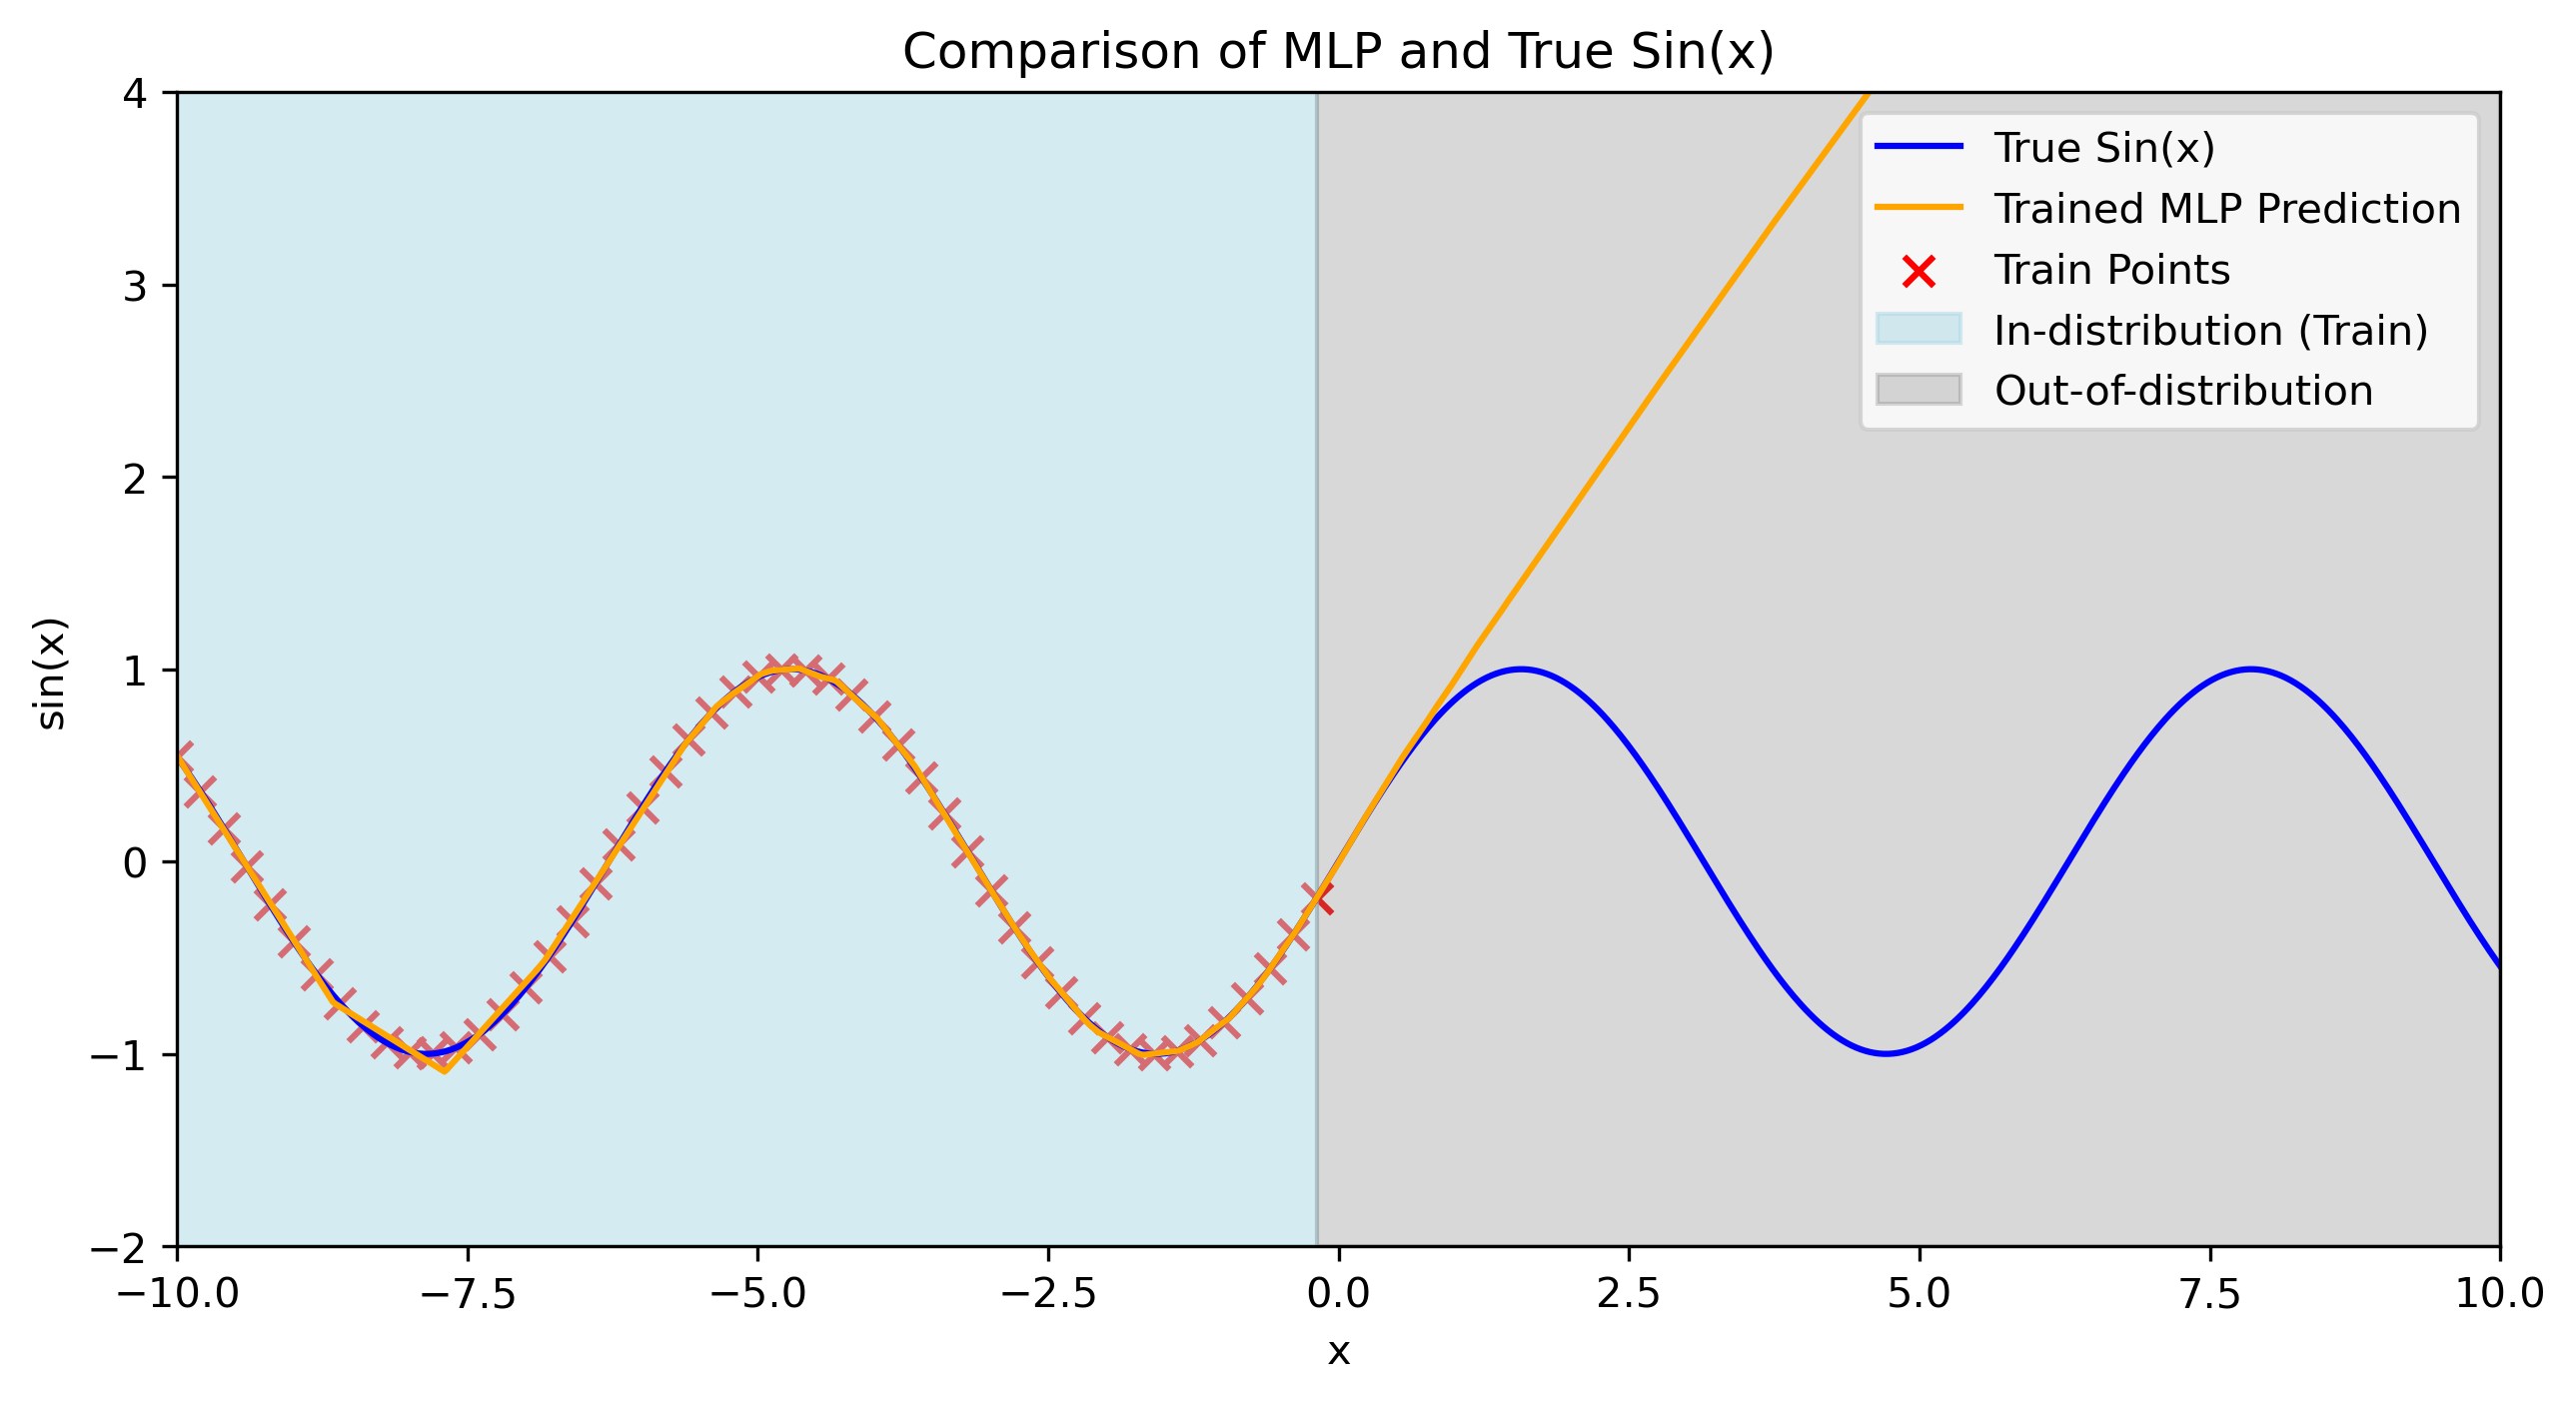
\includegraphics[width=0.9\textwidth]{figs/analytic_vs_nn_inductive_bias.png}
    \caption{Neural network prediction (one layer network with width 100 and ReLU activations)  versus symbolic model for sinusoidal dataset. The symbolic model is $y = sin(x)$.}
    \label{fig:nn_vs_sym_sin}
\end{figure}

\subsection{Symbolic Distillation Framework}
\section{Symbolic Distillation Framework}
The general framework prescribed by the paper for symbolic distillation is as follows:
\begin{itemize}
    \item Design a neural network with an architecture that has a seperable internal structure and an inductive bias that is well suited to modelling the underlying problem.
    \item Train the model with regularisation techniques that encourage the network to learn a low-dimensional representation of the data.
    \item Replace a learned component of the neural network with a symbolic model that approximates that component's output.
    \item Retrain the neural network and repeat the process until all components of the neural network have been replaced with low dimensional symbolic models.
\end{itemize}

% Why even add NNs - factorisation of the search space.
This framework may prompt the question: what is the necessity of employing neural networks initially? Why not directly utilise symbolic regression? The issue arises from the high dimensionality of modern datasets, which renders the application of symbolic regression, essentially a brute-force search over the space of all possible equations, computationally infeasible. To illustrate this point and the motivation behind this work, consider the problem of discovering a force law from a dataset of observed instantaneous accelerations of particles $\mathbf{a}_i \in \mathbb{R}^n$ and their positions $\mathbf{x}_i \in \mathbb{R}^n$. Assume a force law of the form $\mathbf{f}_{ij} = -k |\mathbf{x}_i - \mathbf{x}_j|$, with $\mathbf{a}_i = \frac{\mathbf{F}_i}{m_i}$, where $\mathbf{F}_i = \sum_j \mathbf{f}_{ij}$. To learn symbolic models for the acceleration $\textbf{p}(\textbf{x})$ and the pairwise force $\textbf{q}(\textbf{x})$, one can apply the inductive bias $\textbf{a}_i = \textbf{p}(\sum_j \textbf{q}(\textbf{x}_i, \textbf{x}_j))$. If the symbolic regression model needs to search $N$ equations to fit a given model, the search space scales as $O(N^2)$. However, if neural networks are first used to approximate the functions $\mathbf{p}(x)$ and $\mathbf{q}(x)$, and symbolic regression is subsequently applied to approximate these neural networks, the models can now be fit independently, reducing the search space to $O(N)$. If the dimensionality of the problem $n$ increases or the force law becomes more complex, the number of equations $N$ required to search also increases significantly. Therefore, this factorization of the search space is essential to make symbolic regression tractable for high-dimensional problems.
\subsection{Graph Neural Networks}
The work in the original paper and this report is primarily related to the class of problems which can be classed as interacting particle problems. This type of problem describes a very broad range of most problems encountered in physics. The graph neural network architecture applies a well suited inductive bias to these problems. This section will briefly describe the fundamental components of the graph neural network architecture and why it is well suited to interacting particle problems.

A graph neural network (GNN) is a specialised architecture designed to operate on graph data structures, where nodes represent particles and edges represent pairwise interactions between particles. In this context, each node has an associated feature vector encoding properties such as position, velocity, mass, and charge. The GNN operates through a scheme of message passing, involving two main components: the edge model ($\phi^e$) and the node model ($\phi^v$).
\paragraph*{Edge Model ($\phi^e$):}
   \begin{itemize}
       \item The edge model is applied to each edge $k$ in the graph.
       \item It takes as input the feature vectors of the two nodes $\mathbf{x}_i,\mathbf{x}_j$, connected by the edge.
       \item Formally, $\phi^e : \mathbb{R}^{d_v} \times \mathbb{R}^{d_v} \rightarrow \mathbb{R}^{d_e}$, where $d_v$ is the dimensionality of the node feature vectors, and $d_e$ is the dimensionality of the edge model's output, which is called the edge message $\mathbf{e}_k$.
   \end{itemize}

\paragraph*{Node Model ($\phi^v$):}
   \begin{itemize}
       \item Once every edge has an associated edge message, the node model is applied to each node in the graph.
       \item It takes as input the feature vector of the node, $x_i$, and the aggregated edge messages from all inbound edges, $\bar{e_k}$.
       \item Aggregation is performed using a summation operator.
       \item Formally, $\phi^v : \mathbb{R}^{d_v} \times \mathbb{R}^{d_e} \rightarrow \mathbb{R}^{d_v'}$, where $d_v'$ is the dimensionality of the updated node feature vectors.
       \item The output of the node model is the updated node feature vector.
   \end{itemize}

This message-passing process can be repeated for a number of layers, with the output of the final layer being the output of the graph neural network. The computational graph of the GNN is shown in Figure \ref{fig:gnn}, illustrating the interactions between nodes and edges through the edge and node models. The graph neural network is an appropriate inductive bias for a variety of reasons. Firstly, many important forces in physics are defined on pairs of particles, analogous to the edge model in this context. Further, the summation that aggregates messages is analogous to the calculation of the net force on a receiving particle. Hence, the edge function can be interpretted as the application of the force law and the node function as the application of Newton's second law: acceleration equals the net force (the summed message) divided by the mass of the receiving particle. Further, the graph neural network architecture is invariant under particle permutations, which is a desirable property for a model which represents interacting particle problems. It will be the edge and node models of the graph neural network that will be replaced by symbolic models in the symbolic distillation framework. The goal will be to recover the underlying force law for the edge model and Newton's second law for the node model.
\begin{figure}[H]
    \centering
    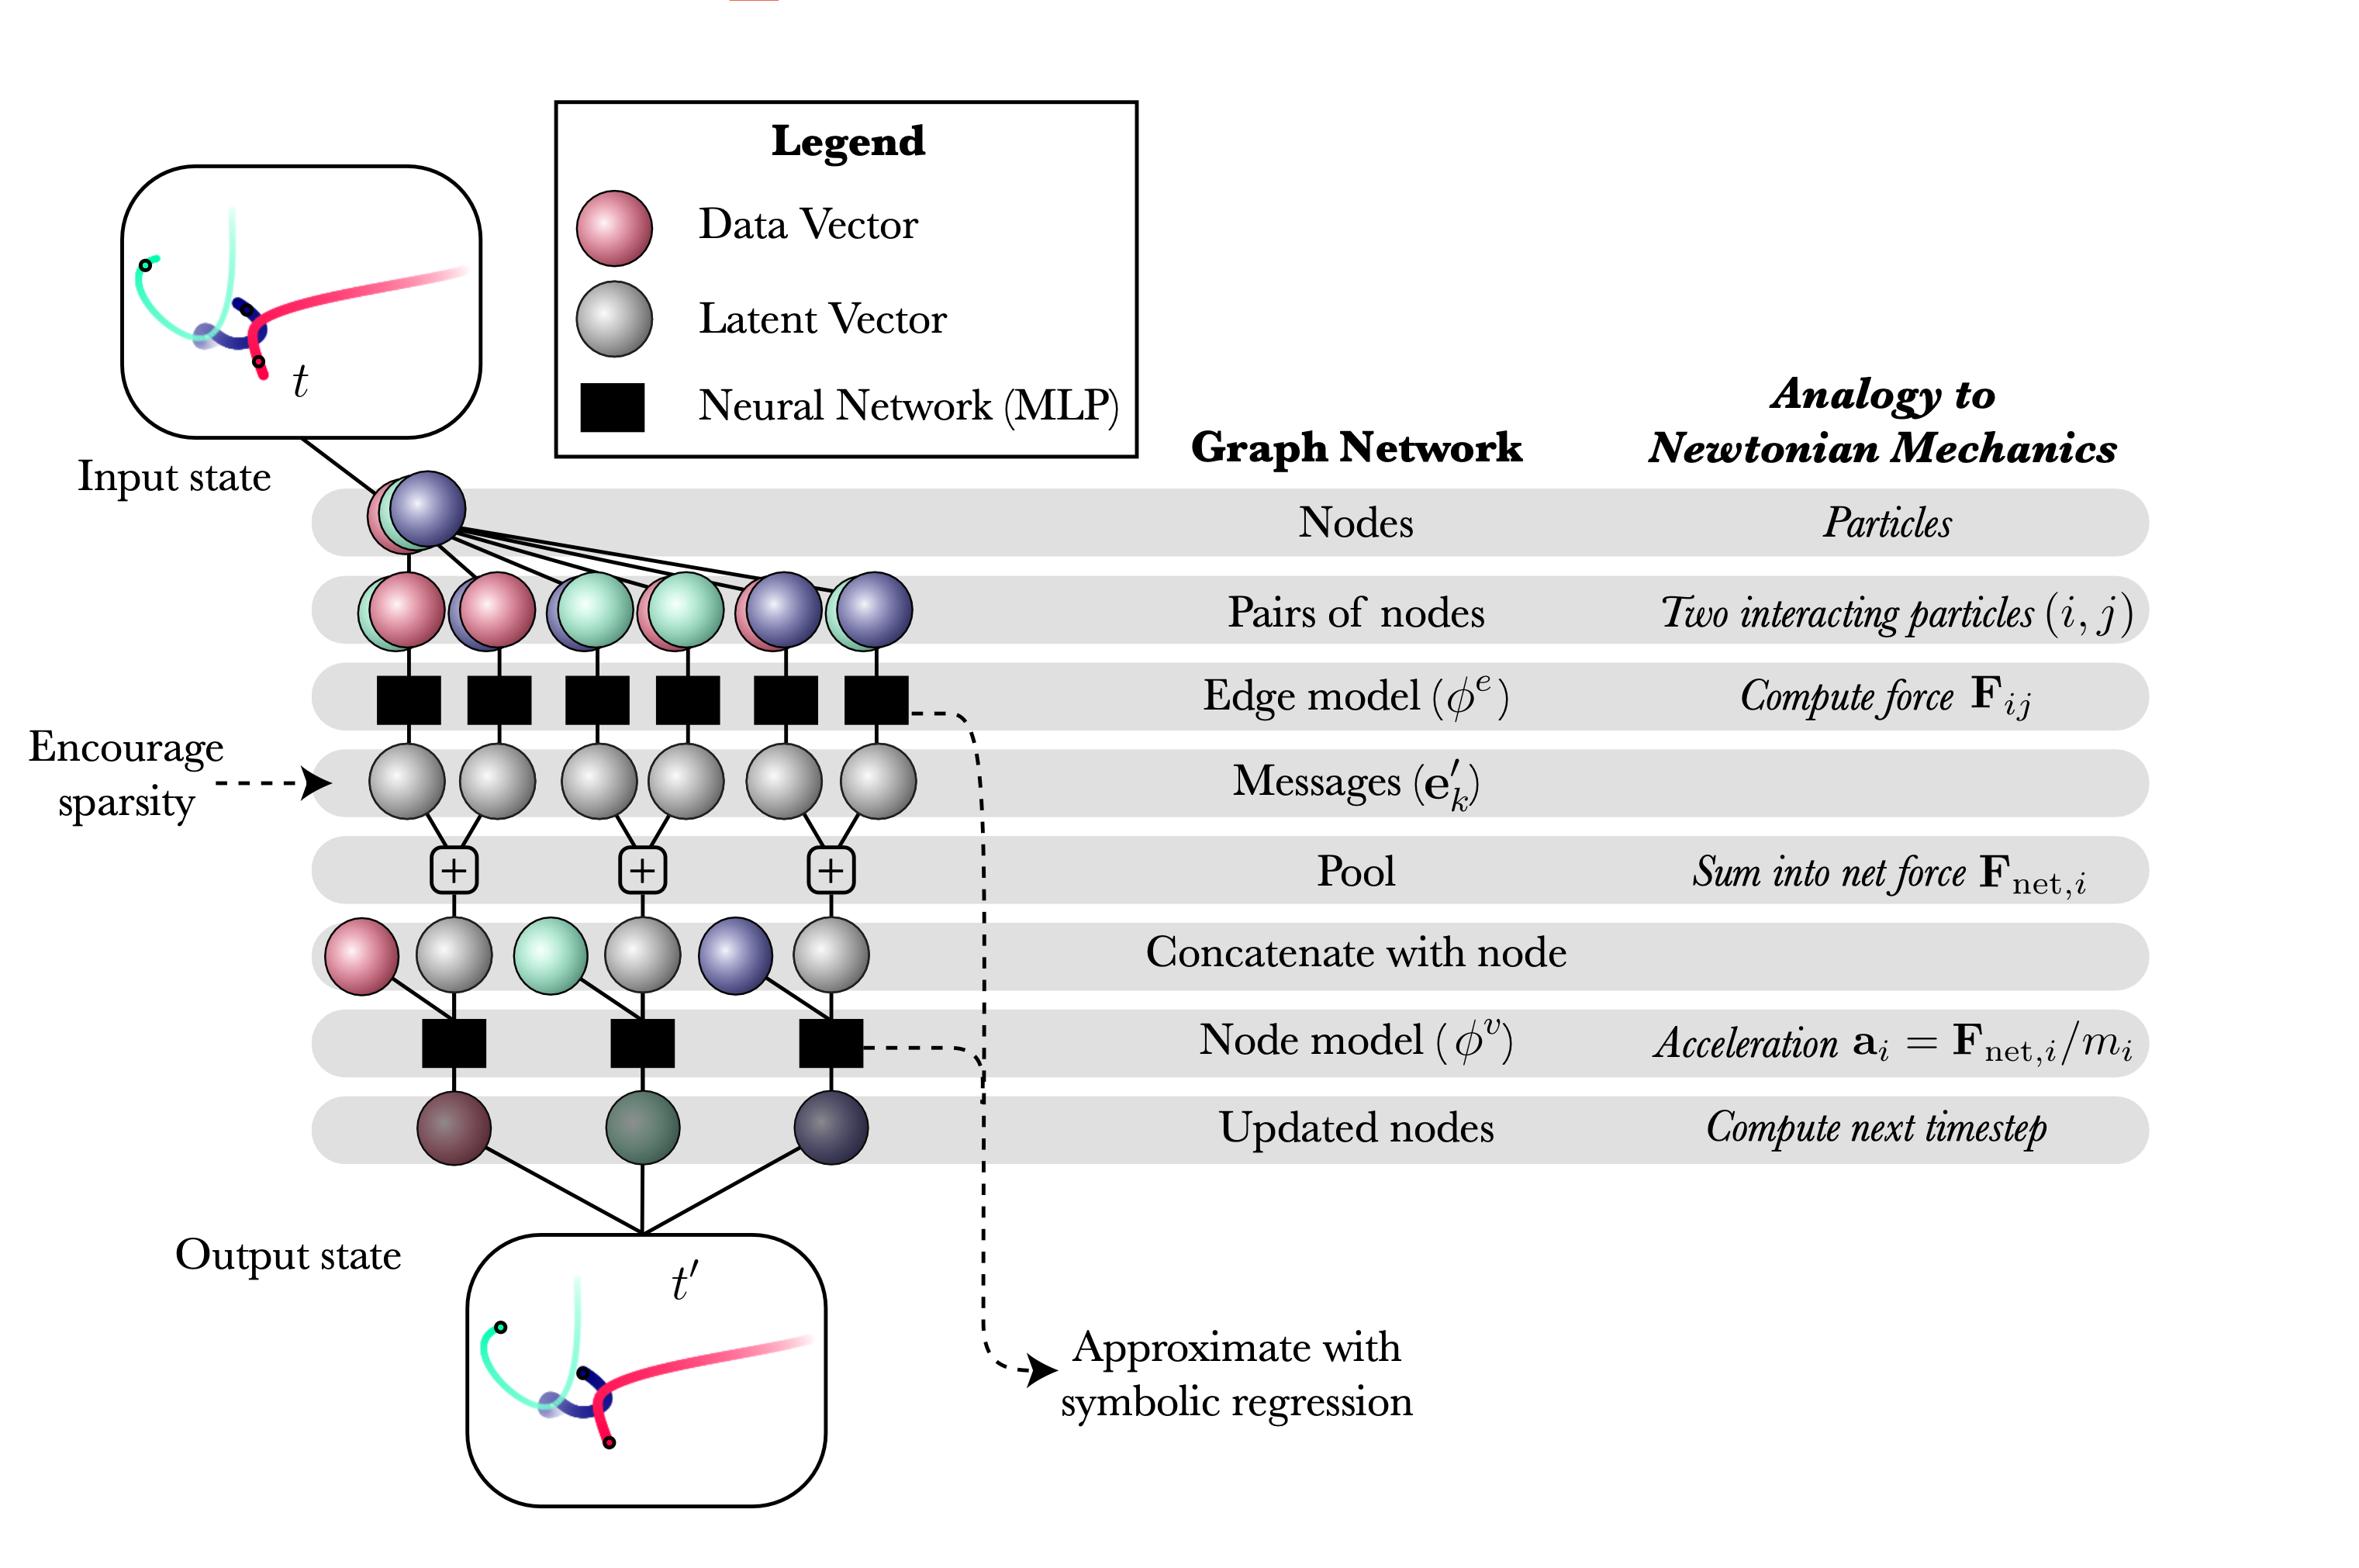
\includegraphics[width=0.9\textwidth]{figs/gnn_diagram.png}
    \caption{Computational graph of the graph neural network architecture. Diagram used from Cranmer et al. \cite{cranmer2020discoveringsymbolicmodelsdeep}}
    \label{fig:gnn}
\end{figure}
% Explain what they are and why they present the appropriate inductive bias for the problem.

% force law interacting particle problems - Fri
% Introduce the data briefly and the pipeline for the problem.
\section{Data}
This section will outline the data used in the experiments and the preprocessing applied. Each dataset used describes an ensemble of N-body particle simulations under a specific force law. From the original paper, the following force laws are investigated:
\begin{itemize}
    \item Spring: \(\textbf{f}_{ij} = -(|\textbf{r}_{ij} - 1|) \hat{\textbf{r}}_{ij}\)
    \item \(\frac{1}{r}\) Orbital force: \(\textbf{f}_{ij} = -\frac{m_i m_j\hat{\textbf{r}}_{ij}}{|\textbf{r}_{ij}|}\)
    \item \(\frac{1}{r^2}\) Orbital force: \(\textbf{f}_{ij} = -\frac{m_i m_j \hat{\textbf{r}}_{ij}}{|\textbf{r}_{ij}|^2}\)
    \item Charge: \(\textbf{f}_{ij} = -\frac{q_i q_j \hat{\textbf{r}}_{ij}}{|\textbf{r}_{ij}|^2}\)
\end{itemize}
Each force law was simulated in 2D and 3D, with 4 and 8 particles respectively. For each experiment, 10000 simulations were run in parallel for 500 time steps. This was split 3:1 to obtain the training and validation set. The test set was generated separately and of the same size as the combined train and validation sets. The initial positions and velocities were sampled from a standard normal distribution, the mass was sampled from a log standard normal distribution and the charge was drawn randomly from the set \(\{-1, 1\}\). 
% Original paper dataset size vs this one 
It is worth noting that the original paper ran each simulation for 1000 time steps, however, to avoid model training times becoming prohibitively long, the simulations were run for half the number of time steps. The step size varies for each simulation due to the differences in scale. It is: 0.005 for \( \frac{1}{r} \), 0.001 for \( \frac{1}{r^2} \), 0.01 for Spring, 0.001 for Charge. The code used for generating the simulations is available in the repository within the \texttt{simulations} directory, sourced from the repository associated with the original paper.
% Preprocessing
\subsection{Preprocessing}
Due to the dependence of orbital and charge force laws on \(r\) raised to a negative power, force values can dramatically increase when particles are close together. This leads to data varying over a scale too extensive for effective neural network learning. To address this, a small epsilon \((10^{-2})\) was added to the denominator to compress \(r\) values into a more manageable range. Nonetheless, velocity and acceleration distributions in some experiments still displayed extremely large outliers. To further refine the data, velocities and accelerations were pruned based on the 0.01\% and 99.99\% percentiles. If any particle in a given timestep exceeded these bounds, the entire graph for that timestep was removed. This process ensured that only timesteps where all particle values were within acceptable limits were retained, enhancing data quality and consistency. Although this method disrupts the temporal continuity of the data, it is important to note that each timestep constitutes a complete graph input for the neural network, and thus time continuity need not be maintained. The impact of this preprocessing is illustrated on the 2D Charge data in Figure \ref{fig:distributions}.

\begin{figure}[H]
    \centering
    \begin{subfigure}{0.9\textwidth}
        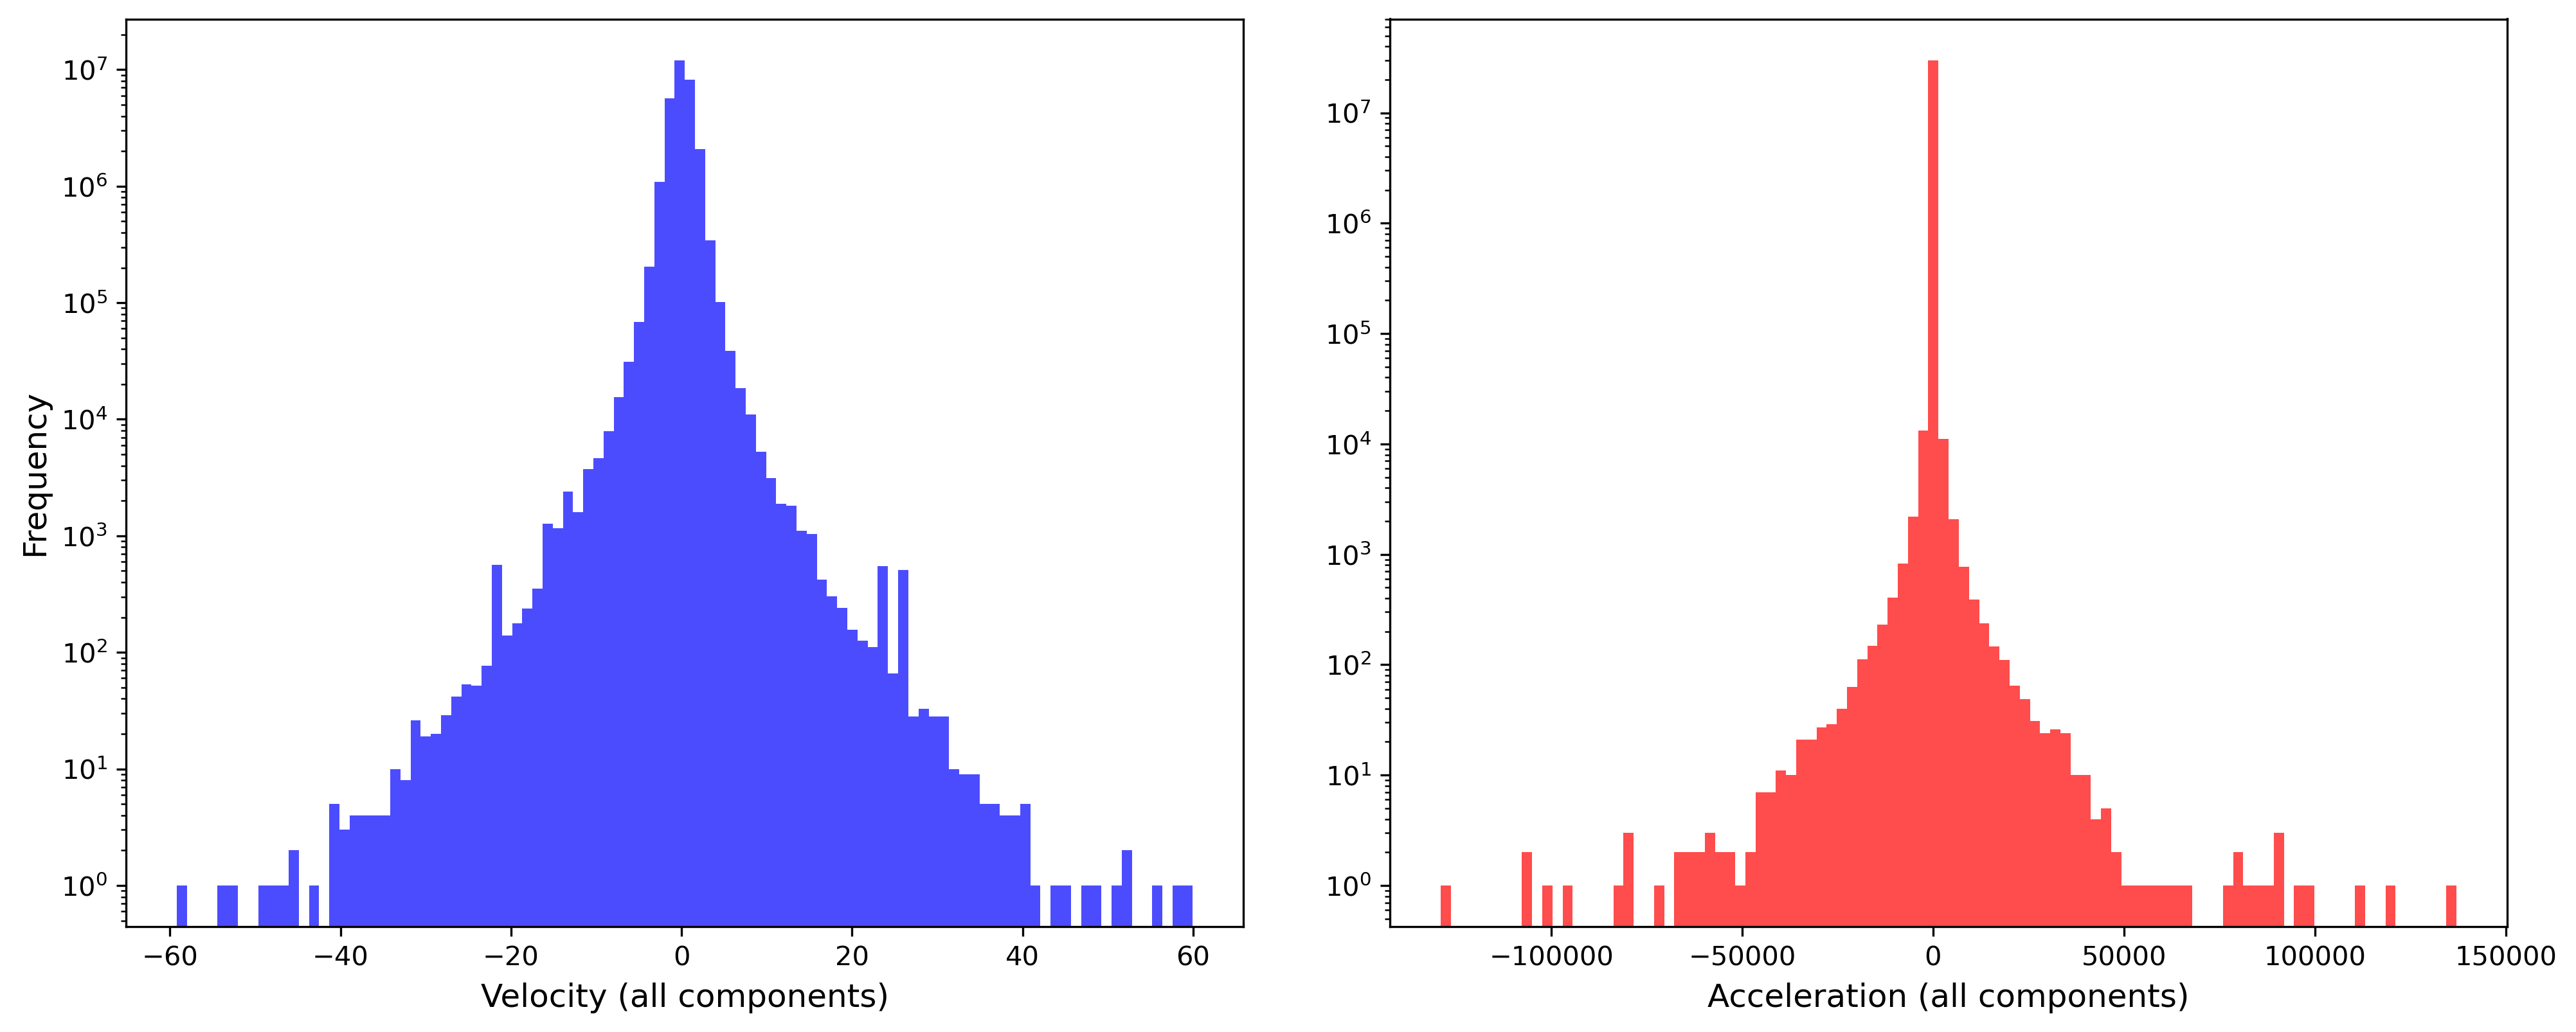
\includegraphics[width=\textwidth]{figs/charge_2_accel_vel_dist_unpruned.png}
        \caption{Charge 2D velocity distribution}
        \label{fig:charge_2_vel_dist_unpruned}
    \end{subfigure}
    \begin{subfigure}{0.9\textwidth}
        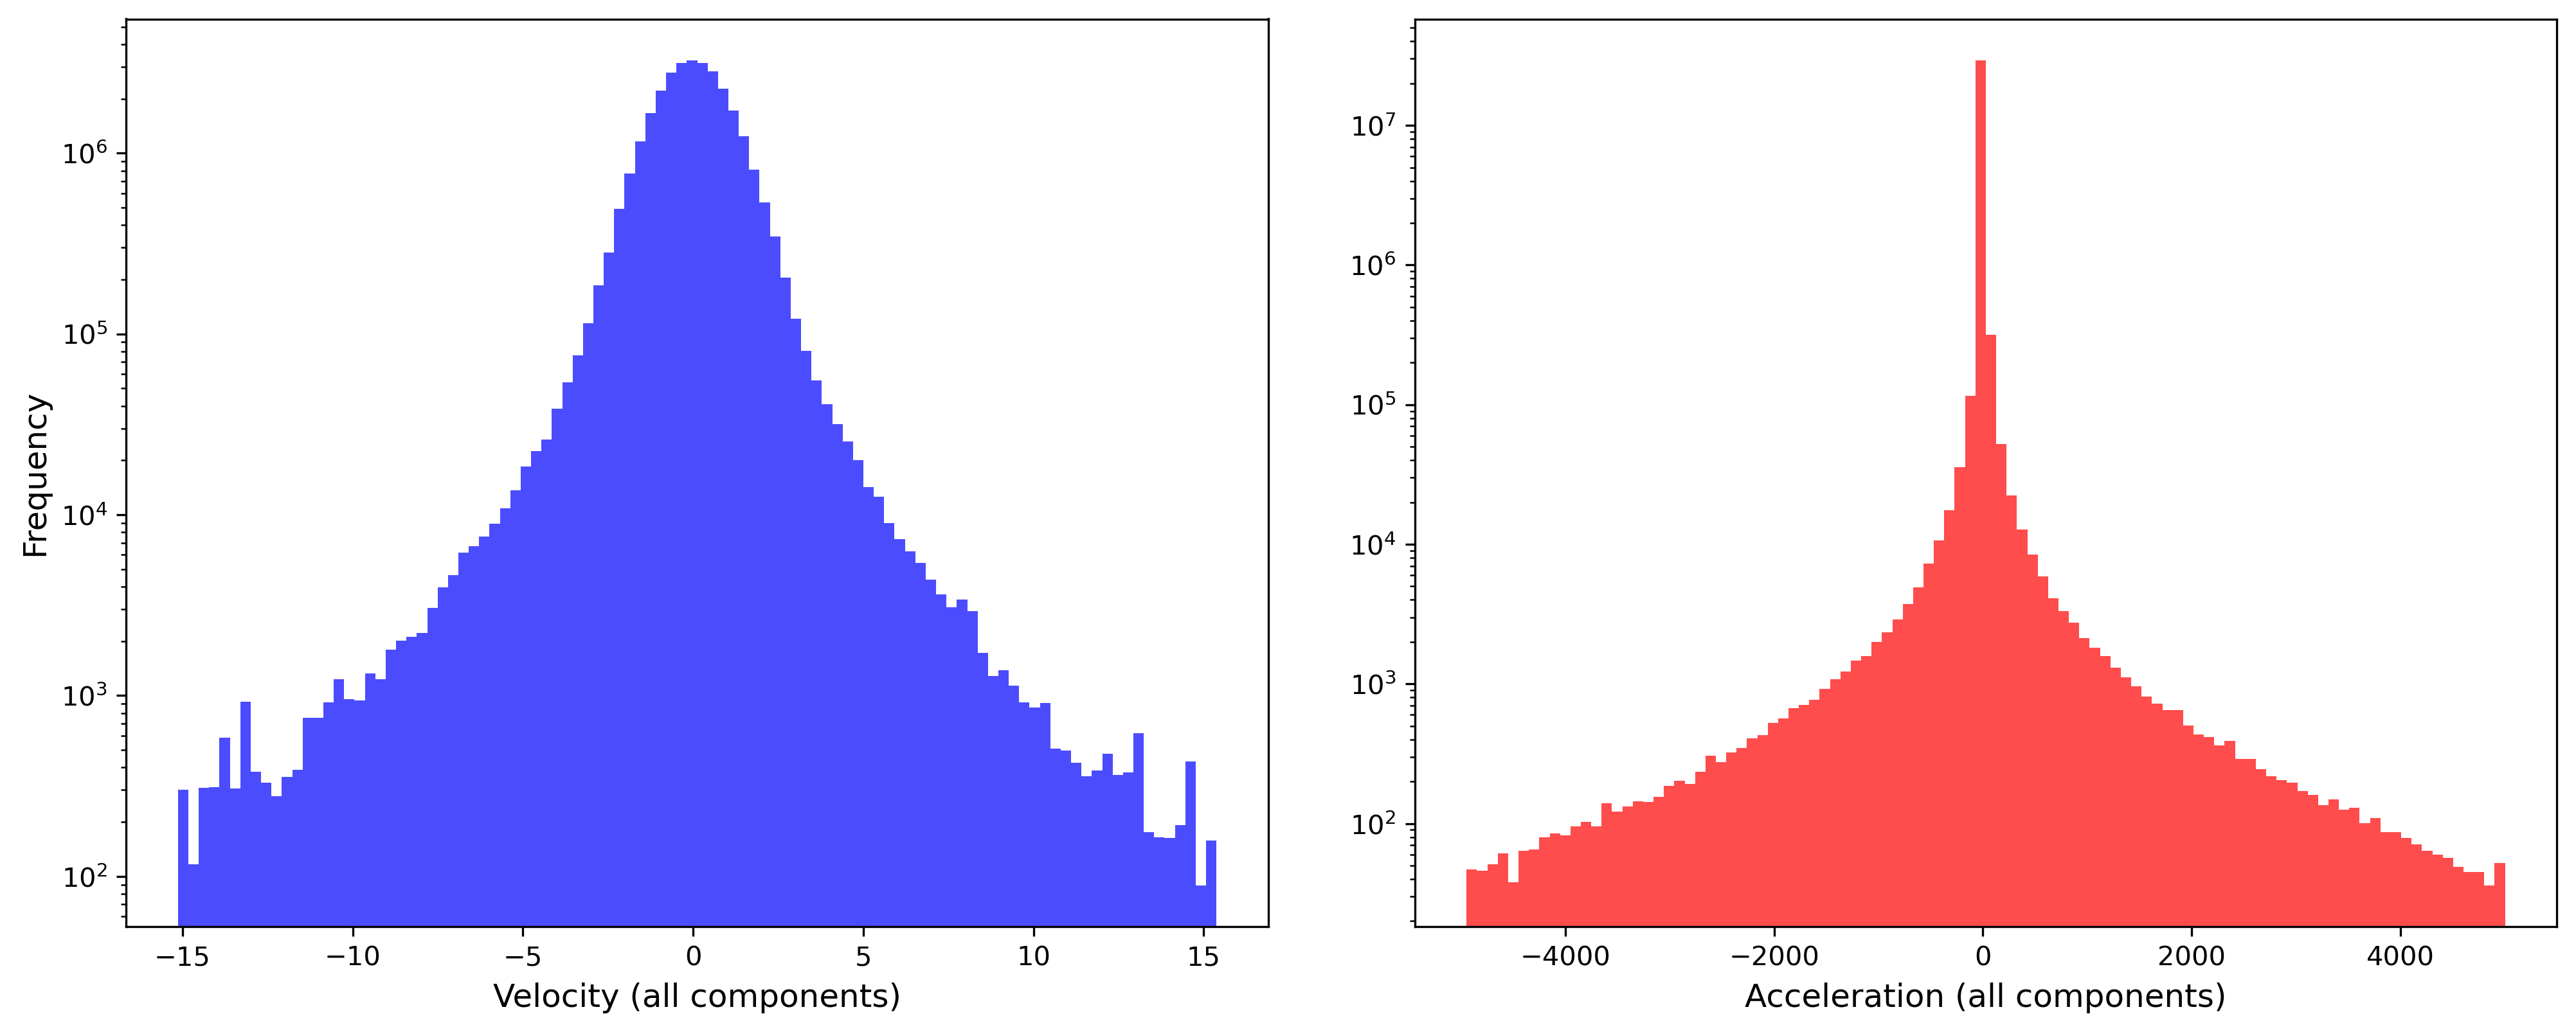
\includegraphics[width=\textwidth]{figs/charge_2_accel_vel_dist_pruned.png}
        \caption{Charge 2D velocity distribution (pruned)}
        \label{fig:charge_2_vel_dist_pruned}
    \end{subfigure}
    \caption{Velocity and acceleration distributions for Charge 2D data before and after preprocessing}
    \label{fig:distributions}
\end{figure}


\section{Method}
This section outlines the method used to train a graph neural network to predict instantaneous accelerations and then distil symbolic models from the trained network.

% Introduce the architecture of the model
\subsection{Model Architecture}
The architecture of the graph neural network (GNN) employed across various training strategies is consistent, except for variations in the output dimension of the edge model. The GNN comprises two multi-layer perceptrons (MLPs): the edge model and the node model.

\paragraph*{Edge Model} This model consists of two hidden layers, each with 300 units and ReLU activation functions. It takes as input the concatenated feature vectors from a pair of nodes connected by an edge in the graph. Each node's feature vector is a vector of size $(2d+2)$ containing the position, velocity, mass, and charge, where $d$ represents the problem's dimensionality (2 or 3). The output dimension of the edge model varies depending on the training strategy, discussed next.

\paragraph*{Node Model} Mirroring the edge model in structure, the node model takes as input the summed edge messages from all inbound edges to a given node, concatenated with the node's feature vector. Its output is a vector of dimension 2 or 3, corresponding to the predicted instantaneous acceleration for the node.
\subsection{Training strategies}
This report investigates 4 of the training strategies outlined in the original paper. The training strategies are as follows: standard, bottleneck, L$_1$ and KL. 

\paragraph*{Standard Strategy}
The standard training strategy serves as the baseline case where the edge message dimensionality is 100 and the loss does not include any regularisation terms. Here the loss function is given by the mean absolute error (MAE) between the predicted and true accelerations.

\paragraph*{KL Strategy}
The KL strategy involves sampling edge messages from a multivariate normal distribution as defined by the output of the edge model, which is now a 200-dimensional vector, with the first 100 dimensions representing the mean and the second 100 dimensions representing the log variance. Additionally, the average Kullback-Leibler divergence penalty over all edge messages, using a standard normal as the prior, is added to the loss. The weight of this term is set to \(1.0 \).

\paragraph*{L$_1$ Strategy}
The L1 strategy is the same as the standard, except it now incorporates the L1 norm of the edge message as a regularisation term, averaged over all edge messages, in the loss. The weight of this term is set to \(1.0 \times 10^{-2}\).

\paragraph*{Bottleneck Strategy}
The bottleneck strategy is the same as the standard, however now aligns the dimensionality of the edge message with the dimensionality of the problem (2 or 3).

\subsection{Model Training}
The network is trained over 100 epochs using the Adam optimizer with an initial learning rate of \(0.001\) and weight decay set to \(1.0 \times 10^{-8}\). It is worth noting that this is half the number of epochs used in the original paper. The learning rate is modulated by the 1cycle learning rate policy \cite{smith2018superconvergence}, which increases the learning rate to a peak of \(0.001\) before gradually decreasing it by a factor of \(100,000\), adhering to a pre-defined schedule. Random translation is used as a form of data augmentation to improve the model's generalisation capabilities. The model is trained on a single NVIDIA A100 GPU.

\subsection{Symbolic Regression of the Network}
% Explain how the sybolic regressor was fit - used less operations than the paper to make it easier to reduce the search space
After training the model end to end, the edge and node model are symbolically distilled using the \texttt{PySR} package \cite{cranmer2023interpretable}. PySR's internal search algorithm is a multi-population evolutionary algorithm, which consists of a unique evolve-simplify-optimise loop, designed for optimisation of unknown scalar constants in newly-discovered empirical expressions. 100 populations were used and evolved for 100 iterations. The operators considered in the fitting process are $ +, -, \times , /$ as well as real constants. Note, this is a subset of the operators used in the original paper when fitting for symbolic models. This was done to reduce the search space and quickly check that the symbolic distillation framework was working as expected.

\subsubsection{Model Selection Criteria}
The best symbolic model is selected by evaluating the MAE and the complexity of the model. The complexity is scored by counting the number of occurrences of each operator, constant, and input variable. PySR outputs several equations at each complexity level. The chosen formula is one that maximises the fractional drop in MAE over an increase in complexity from the next best model.

\subsubsection{Symbolic Distillation of the Edge Model}
Symbolic distillation of the edge model is achieved by sampling inputs and outputs from the test set. The recorded inputs are the concatenated feature vectors of the sending and recieving node, which contain their positions, velocities, masses, and charges. For symbolic distilation of force laws based on relative positions, the positions are transformed into relative displacements ($\Delta x = x_1 - x_2$, similarly for $y$ and $z$ in 3D) and distance ($r = \sqrt{\Delta x^2 + \Delta y^2 + \Delta z^2}$) is calculated. These form the inputs to the symbolic model along with the charges and masses of the two bodies connected by the sampled edge. The recorded outputs are the corresponding 100 dimensional edge messages. For symbolic distilation, the outputs are derived by selecting the $d$ most significant components of the edge message. Where significance is defined by the standard deviation of the component across the sampled edge messages and $d$ refers to the problem's dimensionality (2D or 3D). This process is summarised in Figure \ref{fig:edge_model_symbolic_distillation}. In the original paper, 5000 samples are collected from the test set, however in this analysis 1000 samples are used to reduce the computational cost of performing symbolic regression.

\begin{figure}[H]
    \centering
    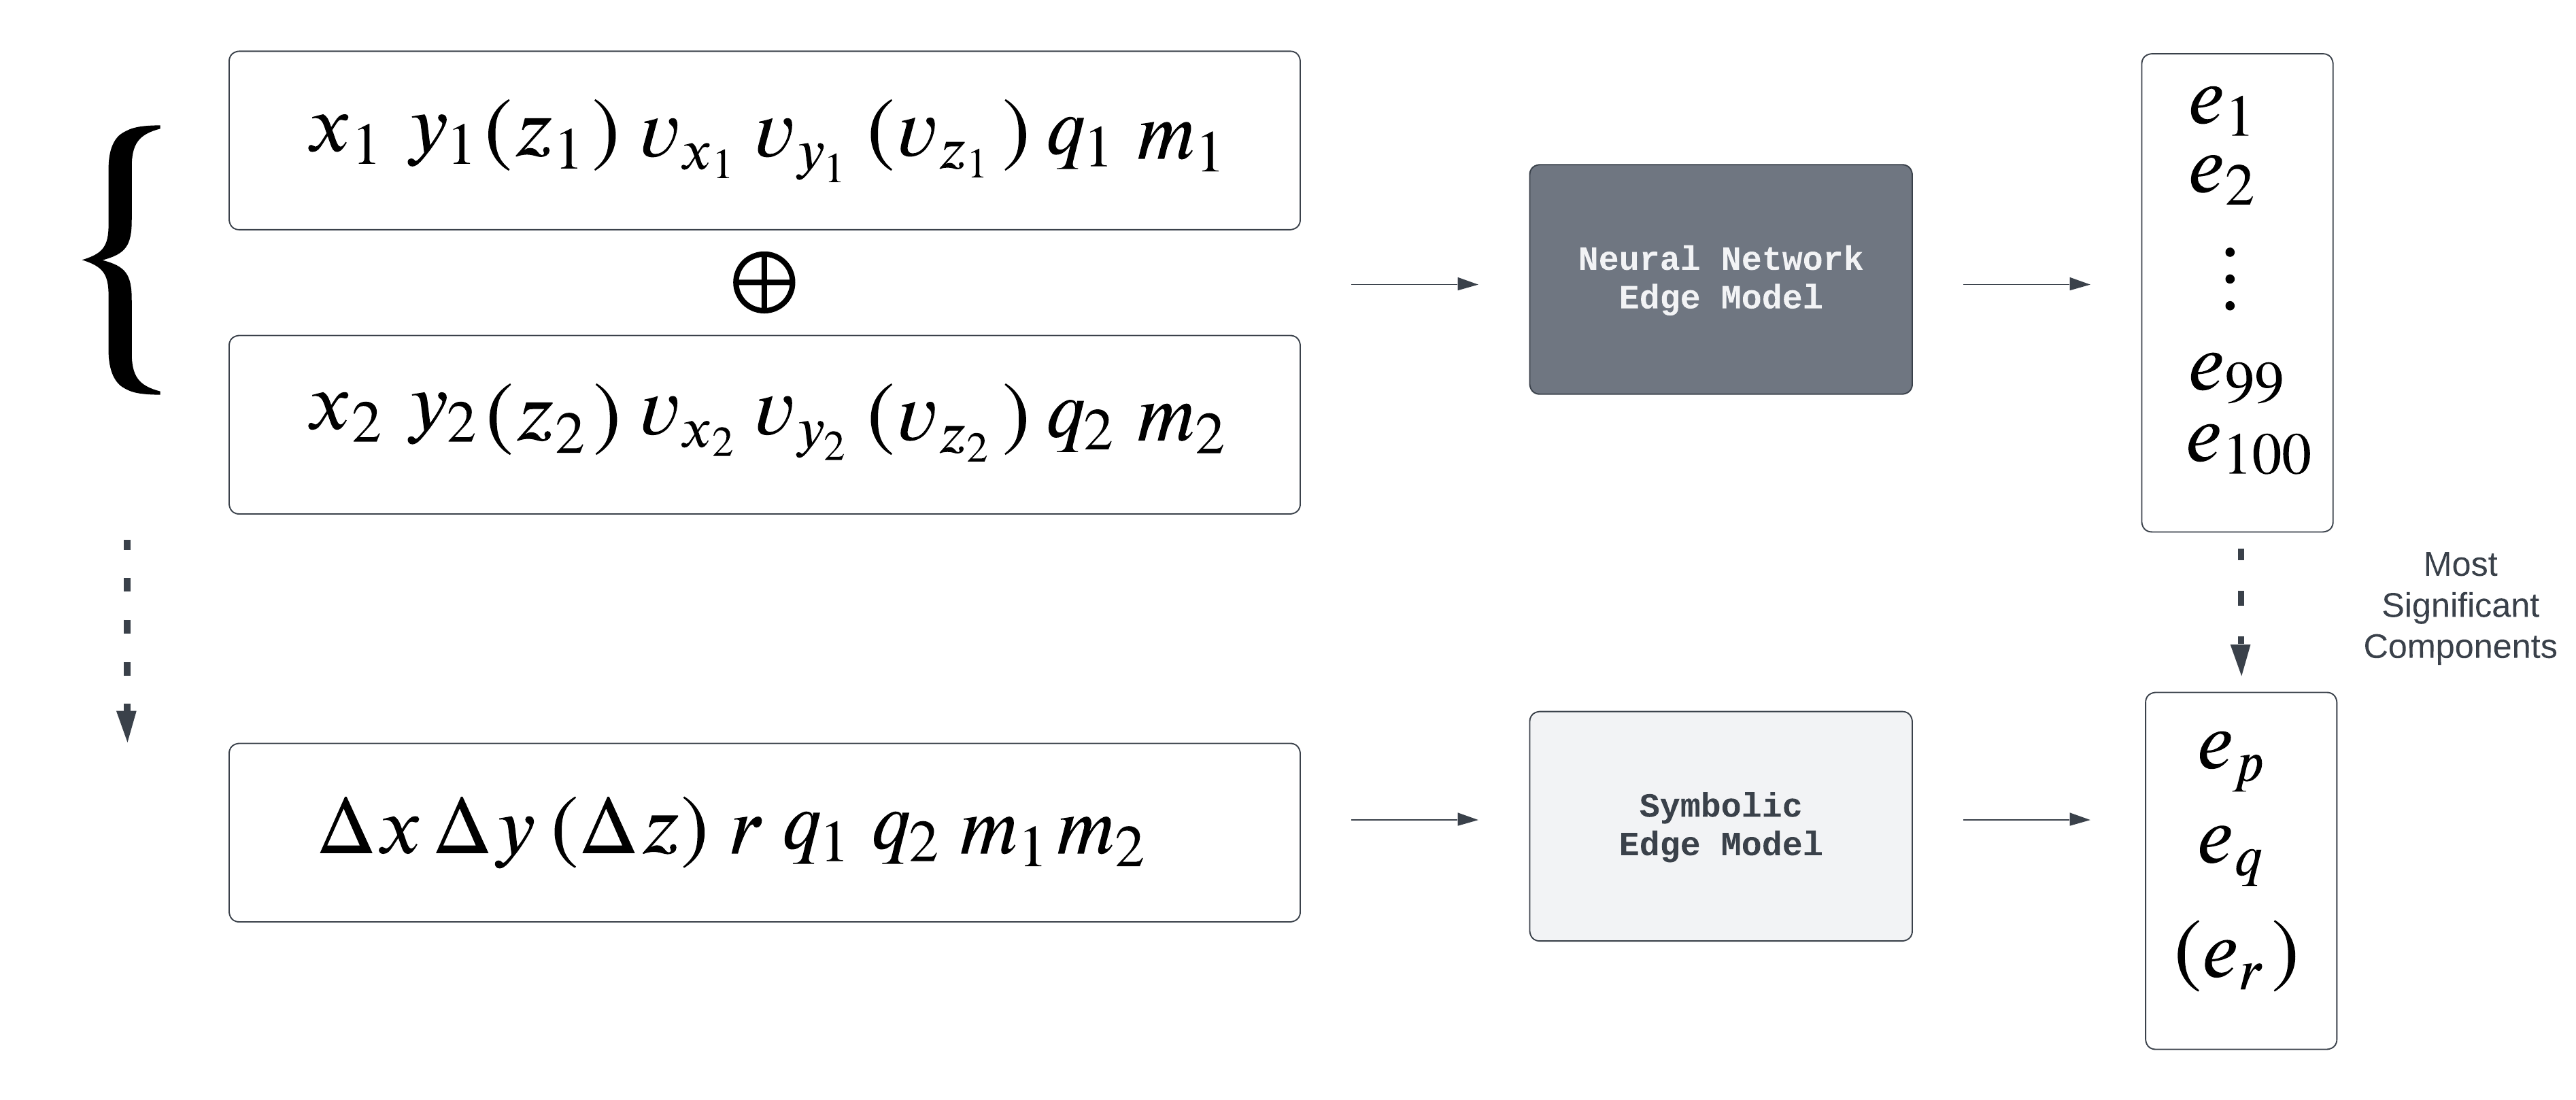
\includegraphics[width=0.9\textwidth]{figs/edge_distillation.png}
    \caption{Symbolic distillation of the edge model.}
    \label{fig:edge_model_symbolic_distillation}
\end{figure}
\subsubsection{Symbolic Distillation of the Node Model}
The symbolic distillation of the node model is similar to that of the edge model. The recorded inputs are the node's feature vectors along with the aggregated edge messages which are calculated by summing over all the inbound edge messages. For symbolic distillation, only the $d$ most significant components of the aggregated edge message are used. The output of the symbolic model is the instantaneous acceleration of the node. This process is summarised in Figure \ref{fig:node_model_symbolic_distillation}.
\begin{figure}[H]
    \centering
    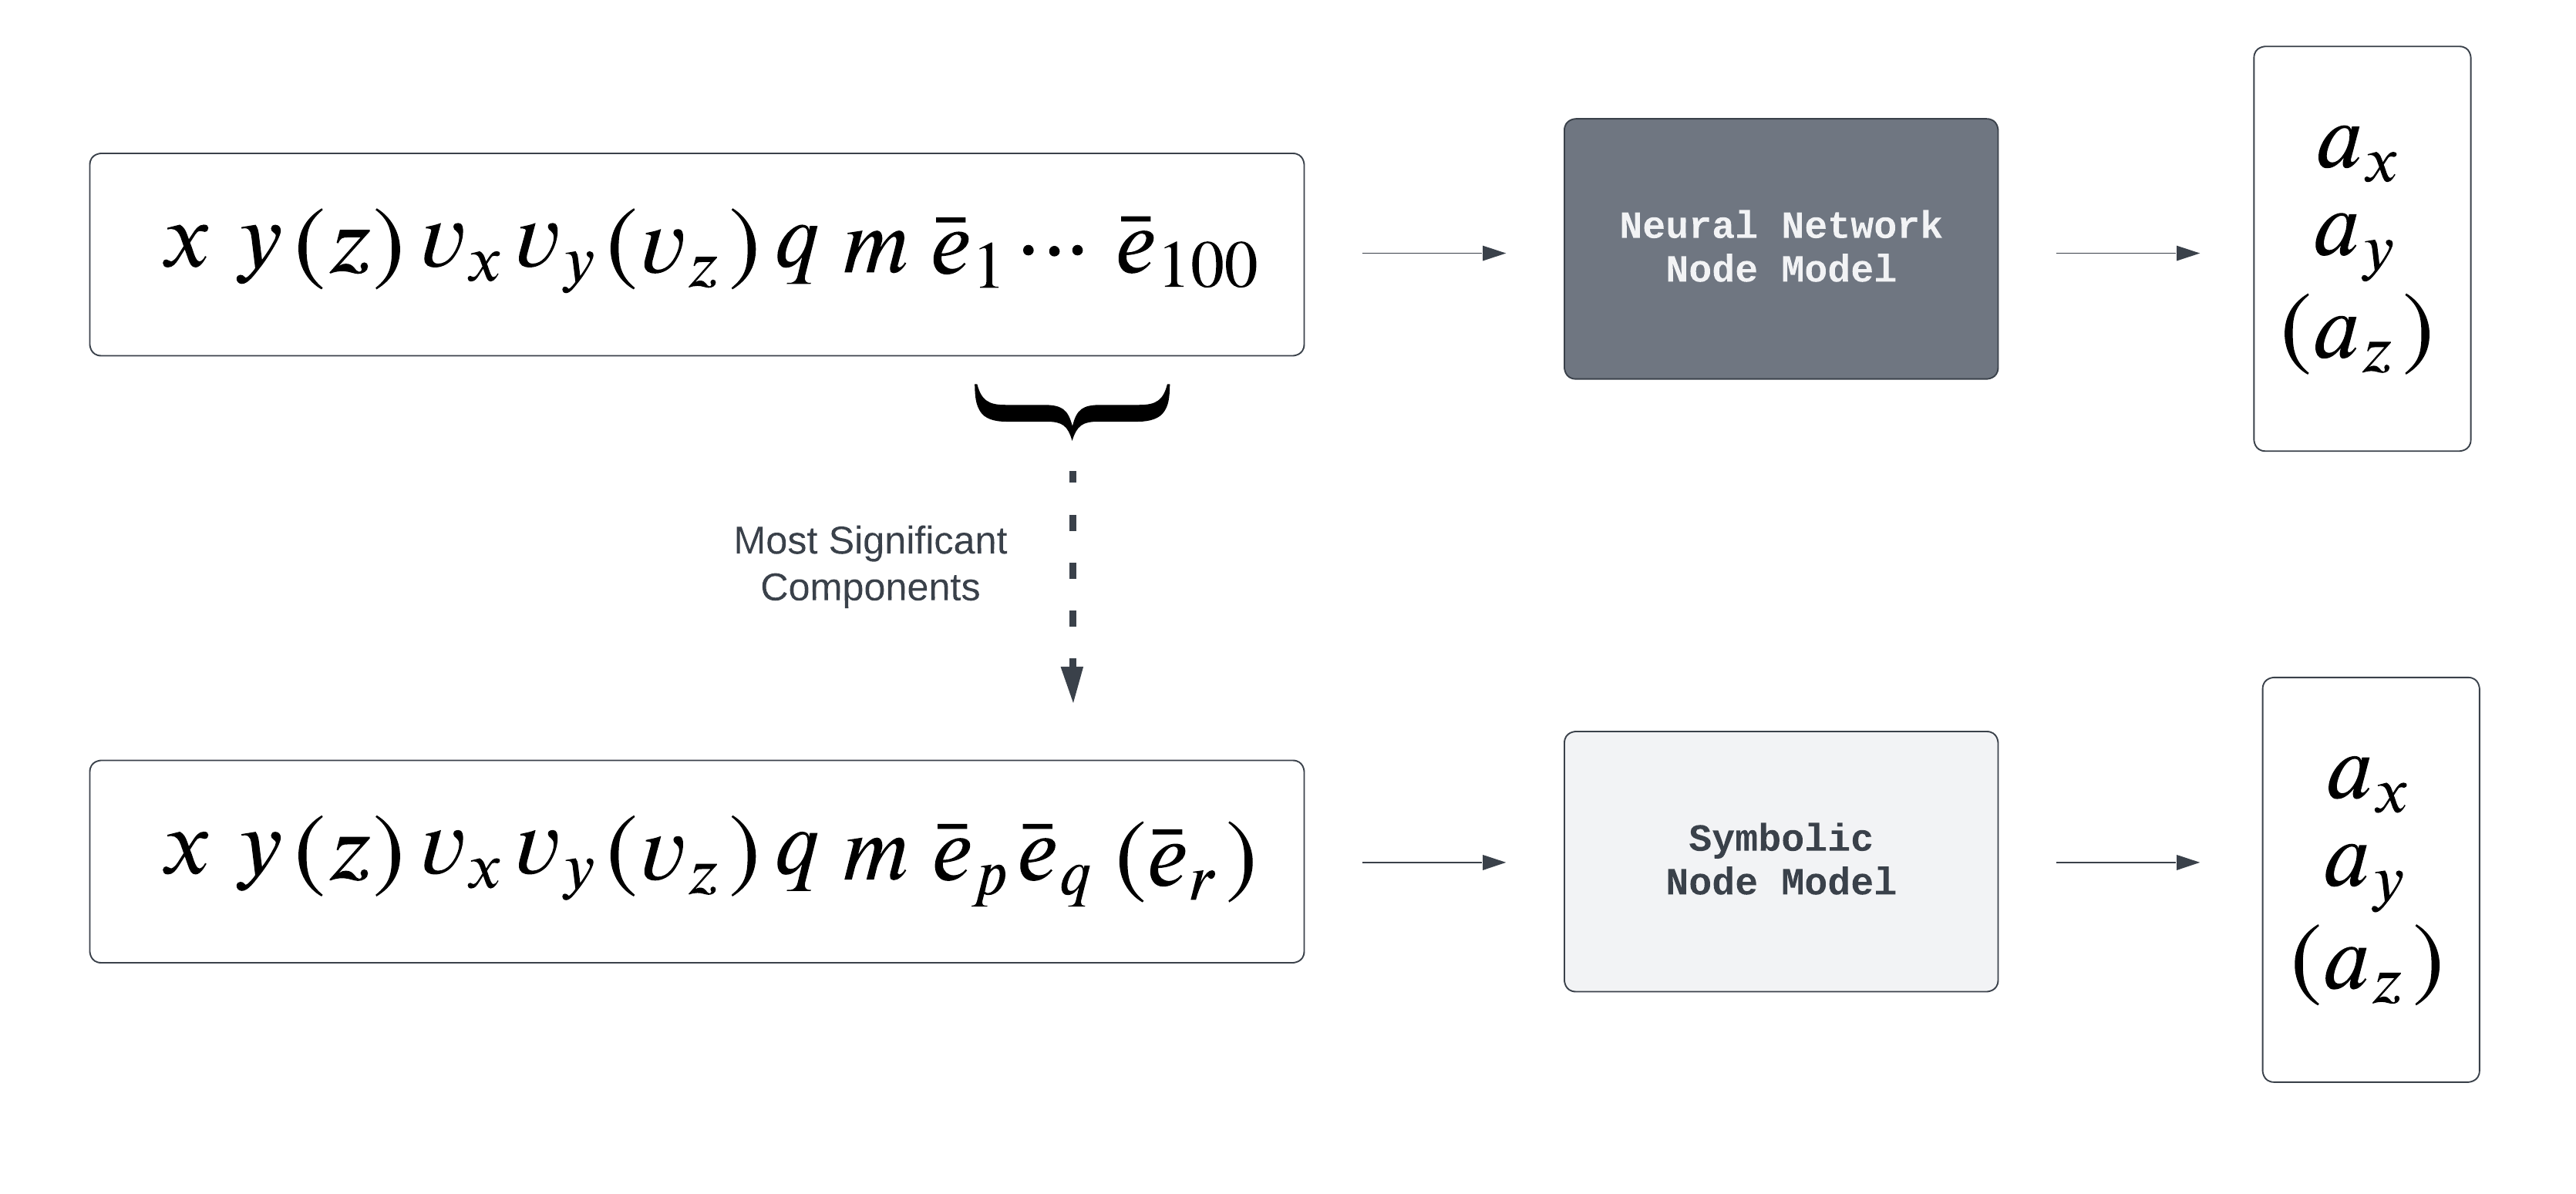
\includegraphics[width=0.9\textwidth]{figs/node_distillation.png}
    \caption{Symbolic distillation of the node model.}
    \label{fig:node_model_symbolic_distillation}
\end{figure}

\subsection{Evaluation Criteria}
To evaluate model performance, the mean absolute error (MAE) between the predicted and true accelerations is calculated over the test set. This metric assesses the predictive capabilities of the trained model. Additionally, the fraction of the total standard deviation contained by the top $d$ edge messages is computed to evaluate the compactness of the learnt representations. This metric indicates whether the training resulted in a model that correctly captured the problem's dimensionality. The $R^2$ metric between the significant edge message components and a linear transformation of the true pairwise force is also calculated. The specific linear transformation is found through a minimisation of the mean squared error (MSE) between observed message components and those predicted by a linear combination of force components. This is implemented through using the \texttt{minimize} function from the \texttt{scipy.optimize} module, employing the Powell method. The optimisation only considers the MSE errors within the 90th percentile of their absolute values, thereby reducing the influence of outliers. This is the same method used in the original paper. The appendix of the original paper provides a mathematical argument for why the model would learn a linear transformation of the pairwise force. The trained models are evaluated through symbolically regressing its edge and node models and checking how many components yield a successful reconstruction describing linear transformation of the true pairwise force and Newtons second law respectively. Finally, for experiments where all edge and node model components were successfully distilled, the symbolic models are compared to the neural networks by evaluating the MAE loss on the test set.

\section{Results}
% Check that if while the edge model might not always be pairwise force, the node model should always just be returning aggr or a scaled version since nns like to learn identity funcs. Cool talking point

\subsection{Model Performance}
The first set of results to be presented are the mean absolute error (MAE) loss on the test set for each simulation. The results are presented in Table \ref{tab:mae_table_with_std}. Two conclusions can be arrived at from this set of results. Firstly, that the KL is the worst by a significant margin as it always has an MAE and standard deviation value that is atleast an order of magnitude larger than those given by the other strategies. The second observation is that while the bottleneck strategy gives the best performance in five out of eight simulations, the margin by which it leads is minimal. This suggests that the other strategies exhibit comparable efficacy in optimising for MAE, with no clear dominant strategy across the board.
\begin{table}[H]
    \centering
    \begin{tabular}{lcccc}
    \hline
    Sim & Standard & Bottleneck & L$_1$ & KL \\
    \hline
    Charge-3 & \textbf{0.110} $\pm$ 0.015 & \textbf{0.140} $\pm$ 0.022 & 0.157 $\pm$ 0.019 & 3.325 $\pm$ 0.168 \\
    Charge-2 & \textbf{0.466} $\pm$ 0.211 & \textbf{0.462} $\pm$ 0.186 & \textbf{0.483} $\pm$ 0.178 & 3.267 $\pm$ 0.417 \\
    r$^{-2}$-3 & \textbf{0.1753} $\pm$ 0.042 & \textbf{0.1746} $\pm$ 0.043 & \textbf{0.2128} $\pm$ 0.050 & 3.8264 $\pm$ 0.264 \\
    r$^{-2}$-2 & \textbf{0.475} $\pm$ 0.169 & \textbf{0.461} $\pm$ 0.167 & \textbf{0.450} $\pm$ 0.142 & 4.0380 $\pm$ 0.557 \\
    r$^{-1}$-3 & 0.0283 $\pm$ 0.003 & \textbf{0.0261} $\pm$ 0.003 & 0.0408 $\pm$ 0.004 & 3.251 $\pm$ 0.101 \\
    r$^{-1}$-2 & 0.0254 $\pm$ 0.005 & \textbf{0.0238} $\pm$ 0.005 & 0.0326 $\pm$ 0.004 & 2.3365 $\pm$ 0.147 \\
    Spring-3 & \textbf{0.0566} $\pm$ 0.003 & 0.0595 $\pm$ 0.003 & 0.0728 $\pm$ 0.004 & 2.6839 $\pm$ 0.057 \\
    Spring-2 & 0.0200 $\pm$ 0.001 & \textbf{0.0182} $\pm$ 0.001 & 0.0249 $\pm$ 0.001 & 1.7455 $\pm$ 0.066 \\
    \hline
    \end{tabular}
    \caption{Mean Absolute Error (MAE) loss on the test set, presented as mean $\pm$ standard deviation. The best values across different training strategies are shown in bold. Values are highlighted in bold when their confidence intervals overlap with the lowest MAE value for a given simulation.}
    \label{tab:mae_table_with_std}
    \end{table}

For comparison, the MAE values for the original paper are presented in Table \ref{tab:mae_table_original}. Unfortunately the original paper does not provide the spread of the MAE values, so it is not possible to compare the standard deviations of the MAE values. However, the original paper also follows the general trend of the standard, bottleneck and L1 performing similarly, with the KL strategy performing significantly worse. However, as a whole, the MAE values in this report are lower than those in the original paper, this is likely due to the preprocessing steps taken to improve data quality that were not present in the original paper.

\begin{table}[H]
    \centering
    \begin{tabular}{lcccc}
    \hline
    Sim & Standard & Bottleneck & L$_1$ & KL \\
    \hline
    Charge-3 & 1.2  & 0.99  & \textbf{0.94}  & 4.2  \\
    Charge-2 & \textbf{49}  & 50  & 52  & 60  \\
    r$^{-2}$-3 & 4.0 & 3.6  & \textbf{3.4} & 9.8  \\
    r$^{-2}$-2 & 1.6  & 1.6  & \textbf{1.2}  & 9.3  \\
    r$^{-1}$-3 & 0.051 & \textbf{0.050}  & 0.055 & 3.5   \\
    r$^{-1}$-2 & 0.077  & \textbf{0.069}  & 0.079  & 3.5   \\
    Spring-3 & 0.11  & 0.11  & \textbf{0.090}  & 3.8  \\
    Spring-2 & 0.047  & 0.046  & \textbf{0.045}  & 1.7  \\
    \hline
    \end{tabular}
    \caption{Mean Absolute Error (MAE) loss on the test set \textbf{in the original paper}. The best values across different training strategies are shown in bold}
    \label{tab:mae_table_original}
    \end{table}
\subsection{Edge Message $R^2$}
The next set of results presented are the $R^2$ values between significant edge message components and the linearly transformed true pairwise forces (or accelerations), averaged across all components. The results are presented in Table \ref{tab:R2}. For comparison, the $R^2$ values for the original paper are presented in Table \ref{tab:R2_original}. Example scatter plots of the edge message components against the linear transformation of the pairwise force for the different strategies of the spring 2D simulation are shown in Figure \ref{fig:scatter_plots}. The standard strategy in this report is found to have a significantly different value than that in the original paper which finds that in all simulations, it is very close to 0. It is not clear from the original papers results if these values were calculated strictly between the significant edge message components and the pairwise force, or if they also considered the pairwise accelerations. This discrepancy is looked at in more detail in the discussion section.
    \begin{table}[H]
        \centering
        \begin{tabular}{lcccc}
        \hline
        Sim & Standard & Bottleneck & L$_1$ & KL \\
        \hline
        Charge-3 & 0.429 \textbf{(0.990)} & 0.817 (0.788) & 0.683 (0.897) & 0.251 (0.472) \\
        Charge-2 & 0.006 (0.050) & 0.700 \textbf{(0.897)} & 0.006 (0.055) & 0.381 (0.431)\\
        r$^{-2}$-3 & 0.502 (0.955) & 0.518 \textbf{(0.998)} & 0.505 (0.979) & 0.323 (0.564) \\
        r$^{-2}$-2 & 0.001 (0.397) & 0.411 \textbf{(0.985)} & 0.181 (0.528) & 0.291 (0.426) \\
        r$^{-1}$-3 & 0.402 \textbf{(0.999)} & 0.403 \textbf{(0.999)} & 0.364 (0.904) & 0.333 (0.859)\\
        r$^{-1}$-2 & 0.314 (0.962) & 0.324 \textbf{(0.994)} & 0.324 \textbf{(0.994)} & 0.250 (0.835) \\
        Spring-3 & 0.430 \textbf{(1.000)}& 0.430 \textbf{(1.000)} & 0.990 (0.438) & 0.918 (0.532)\\
        Spring-2 & 0.422 (0.999) & 0.999 (0.431) & \textbf{1.000} (0.430) & 0.768 (0.640) \\

        \hline
        \end{tabular}
        \caption{$R^2$ metric between the significant edge message components and a linear transformation of the true pairwise force (and pairwise acceleration shown in brackets). Best value across training strategy shown in bold (for either acceleration or force).}
        \label{tab:R2}
    \end{table}
    \begin{table}[H]
        \centering
        \begin{tabular}{lcccc}
        \hline
        Sim & Standard & Bottleneck & L$_1$ & KL \\
        \hline
        Charge-3 & 0.013 & \textbf{0.980} & 0.002 & 0.425 \\
        Charge-2 & 0.016 & \textbf{0.947} & 0.004 & 0.185 \\
        r$^{-2}$-3 & 0.002 & \textbf{0.994} & 0.977 & 0.214 \\
        r$^{-2}$-2 & 0.004 & 0.993 & \textbf{0.990} & 0.770 \\
        r$^{-1}$-3 & 0.000 & \textbf{1.000} & \textbf{1.000} & 0.332 \\
        r$^{-1}$-2 & 0.000 & \textbf{1.000} & \textbf{1.000} & 0.796 \\
        Spring-3 & 0.036 & 0.995 & \textbf{1.000} & 0.214 \\
        Spring-2 & 0.032 & \textbf{1.000} & \textbf{1.000} & 0.883 \\
        \hline
        \end{tabular}
        \caption{$R^2$ metric between the significant edge message components and a linear transformation of the true pairwise force \textbf{in the original paper}. Best value across training strategy shown in bold.}
        \label{tab:R2_original}
    \end{table}


    \begin{figure}[H]
        \centering
        \begin{subfigure}{0.45\textwidth}
            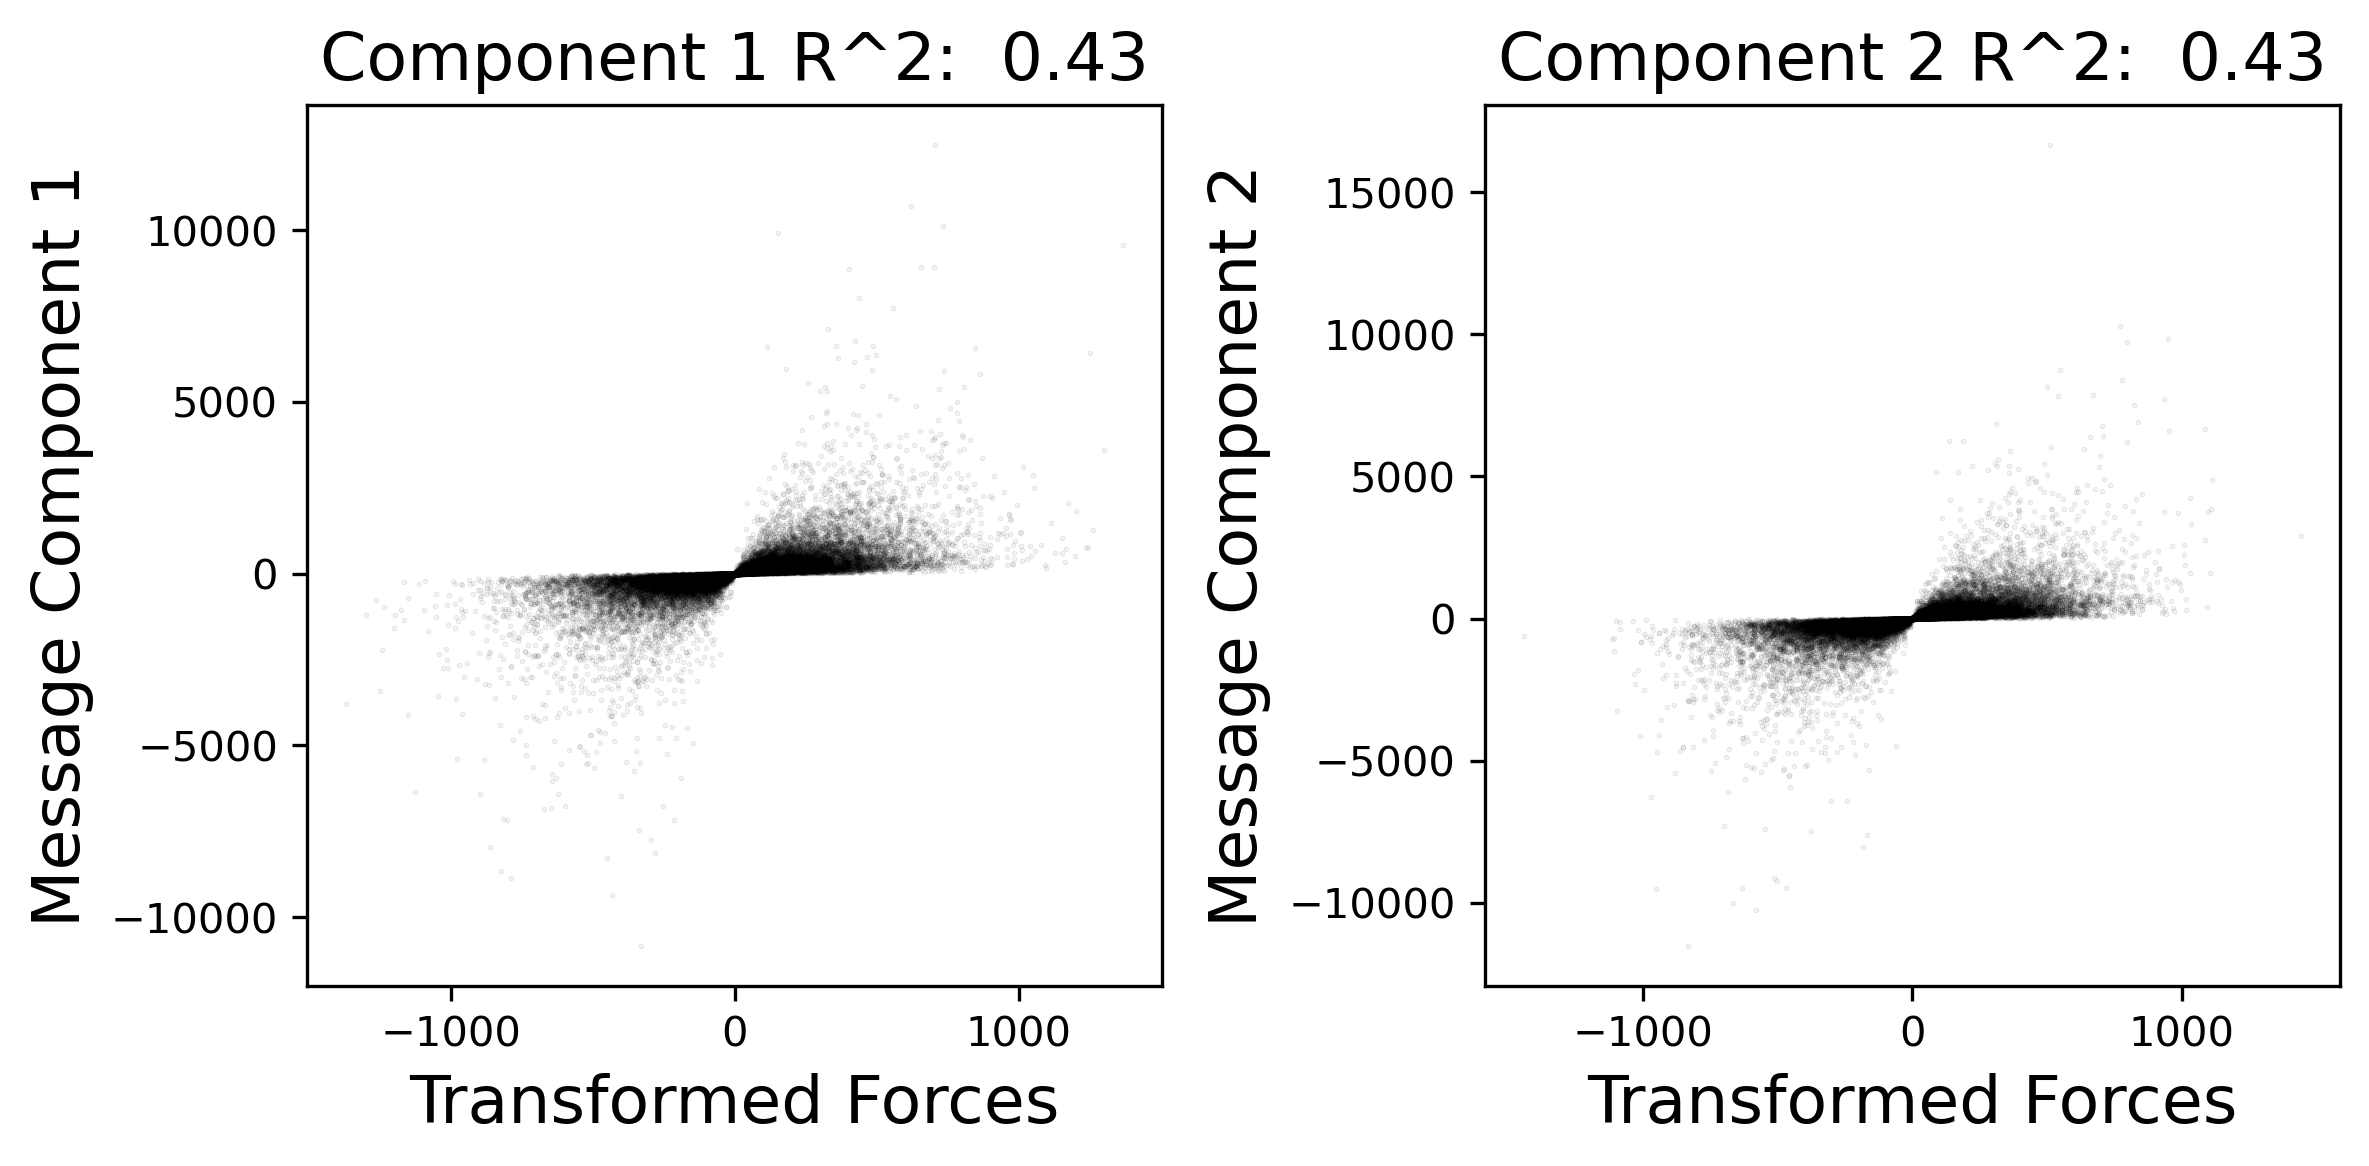
\includegraphics[width=\textwidth]{figs/spring_2d_standard_r2.png}
            \caption{Spring 2D, Standard}
        \end{subfigure}
        \begin{subfigure}{0.45\textwidth}
            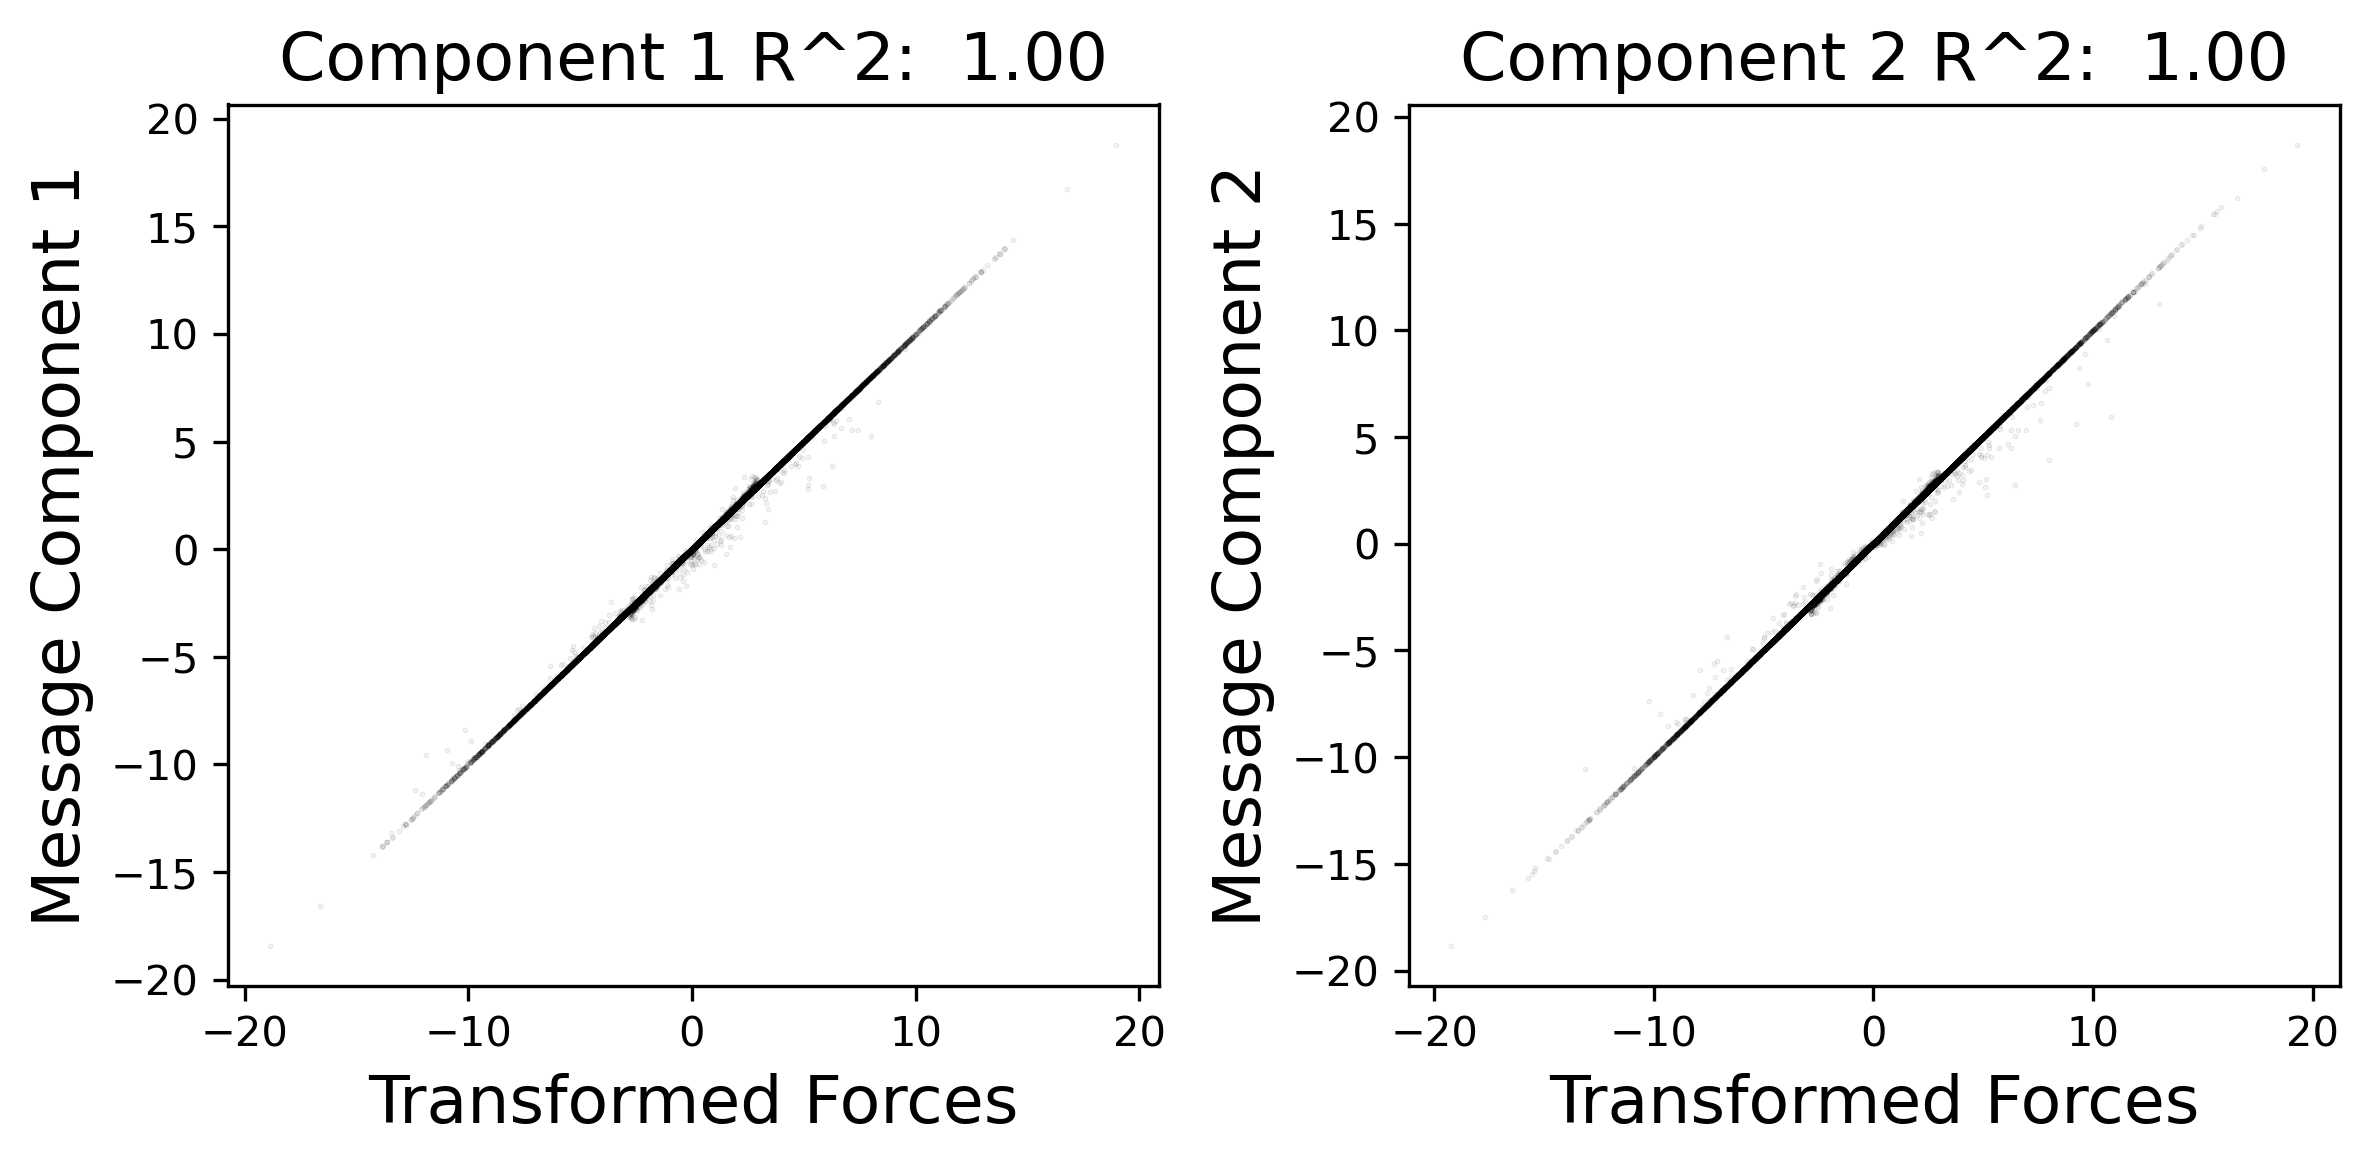
\includegraphics[width=\textwidth]{figs/spring_2d_bottleneck_r2.png}
            \caption{Spring 2D, Bottleneck}
        \end{subfigure}
        
        \begin{subfigure}{0.45\textwidth}
            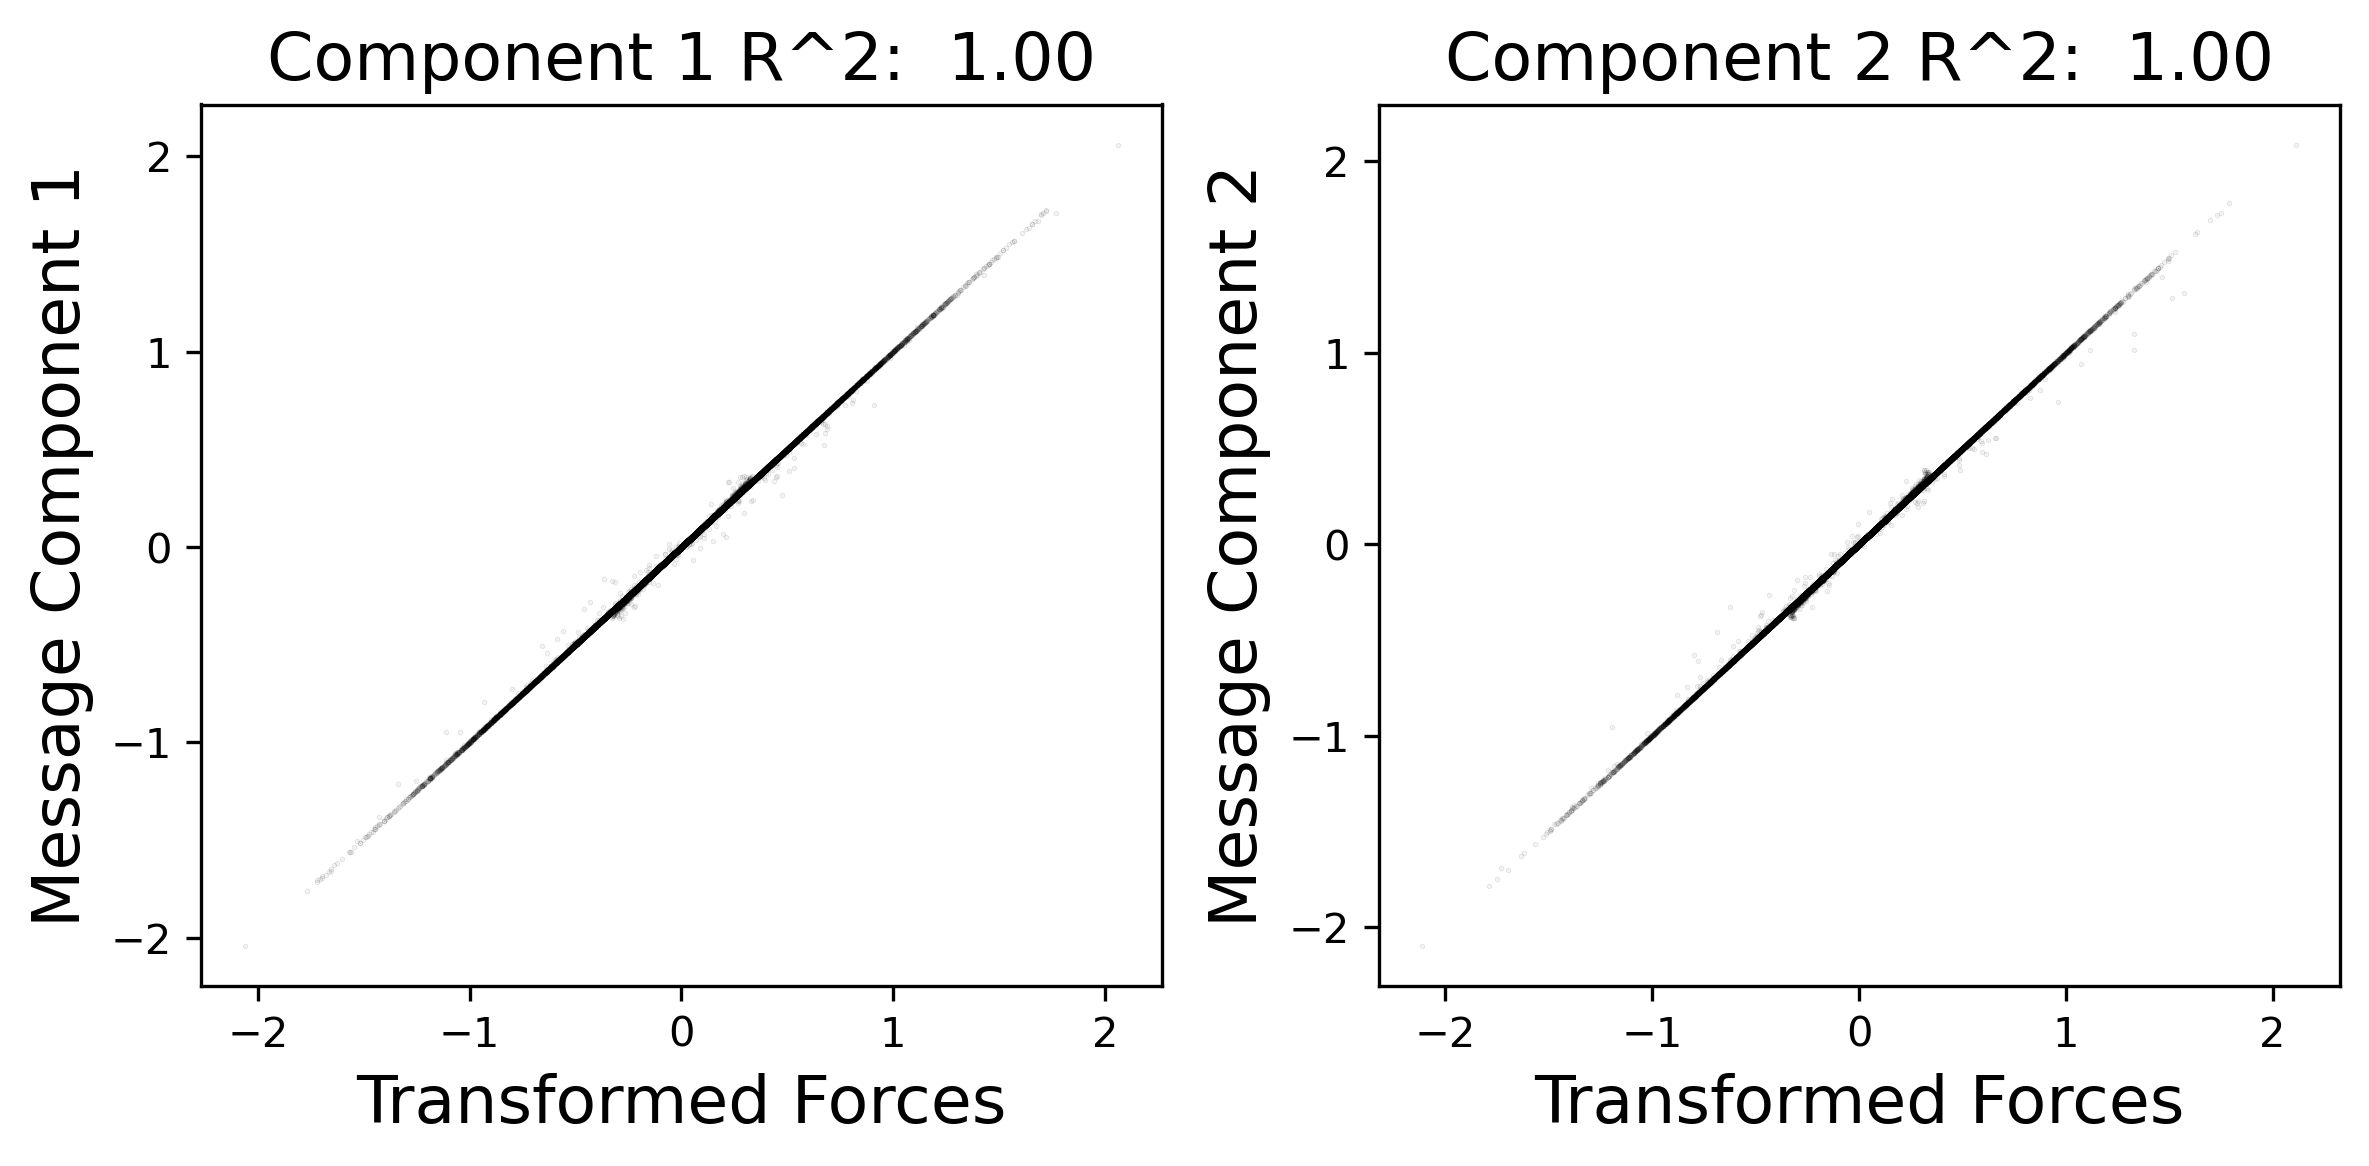
\includegraphics[width=\textwidth]{figs/spring_2d_l1_r2.png}
            \caption{Spring 2D, L$_1$}
        \end{subfigure}
        \begin{subfigure}{0.45\textwidth}
            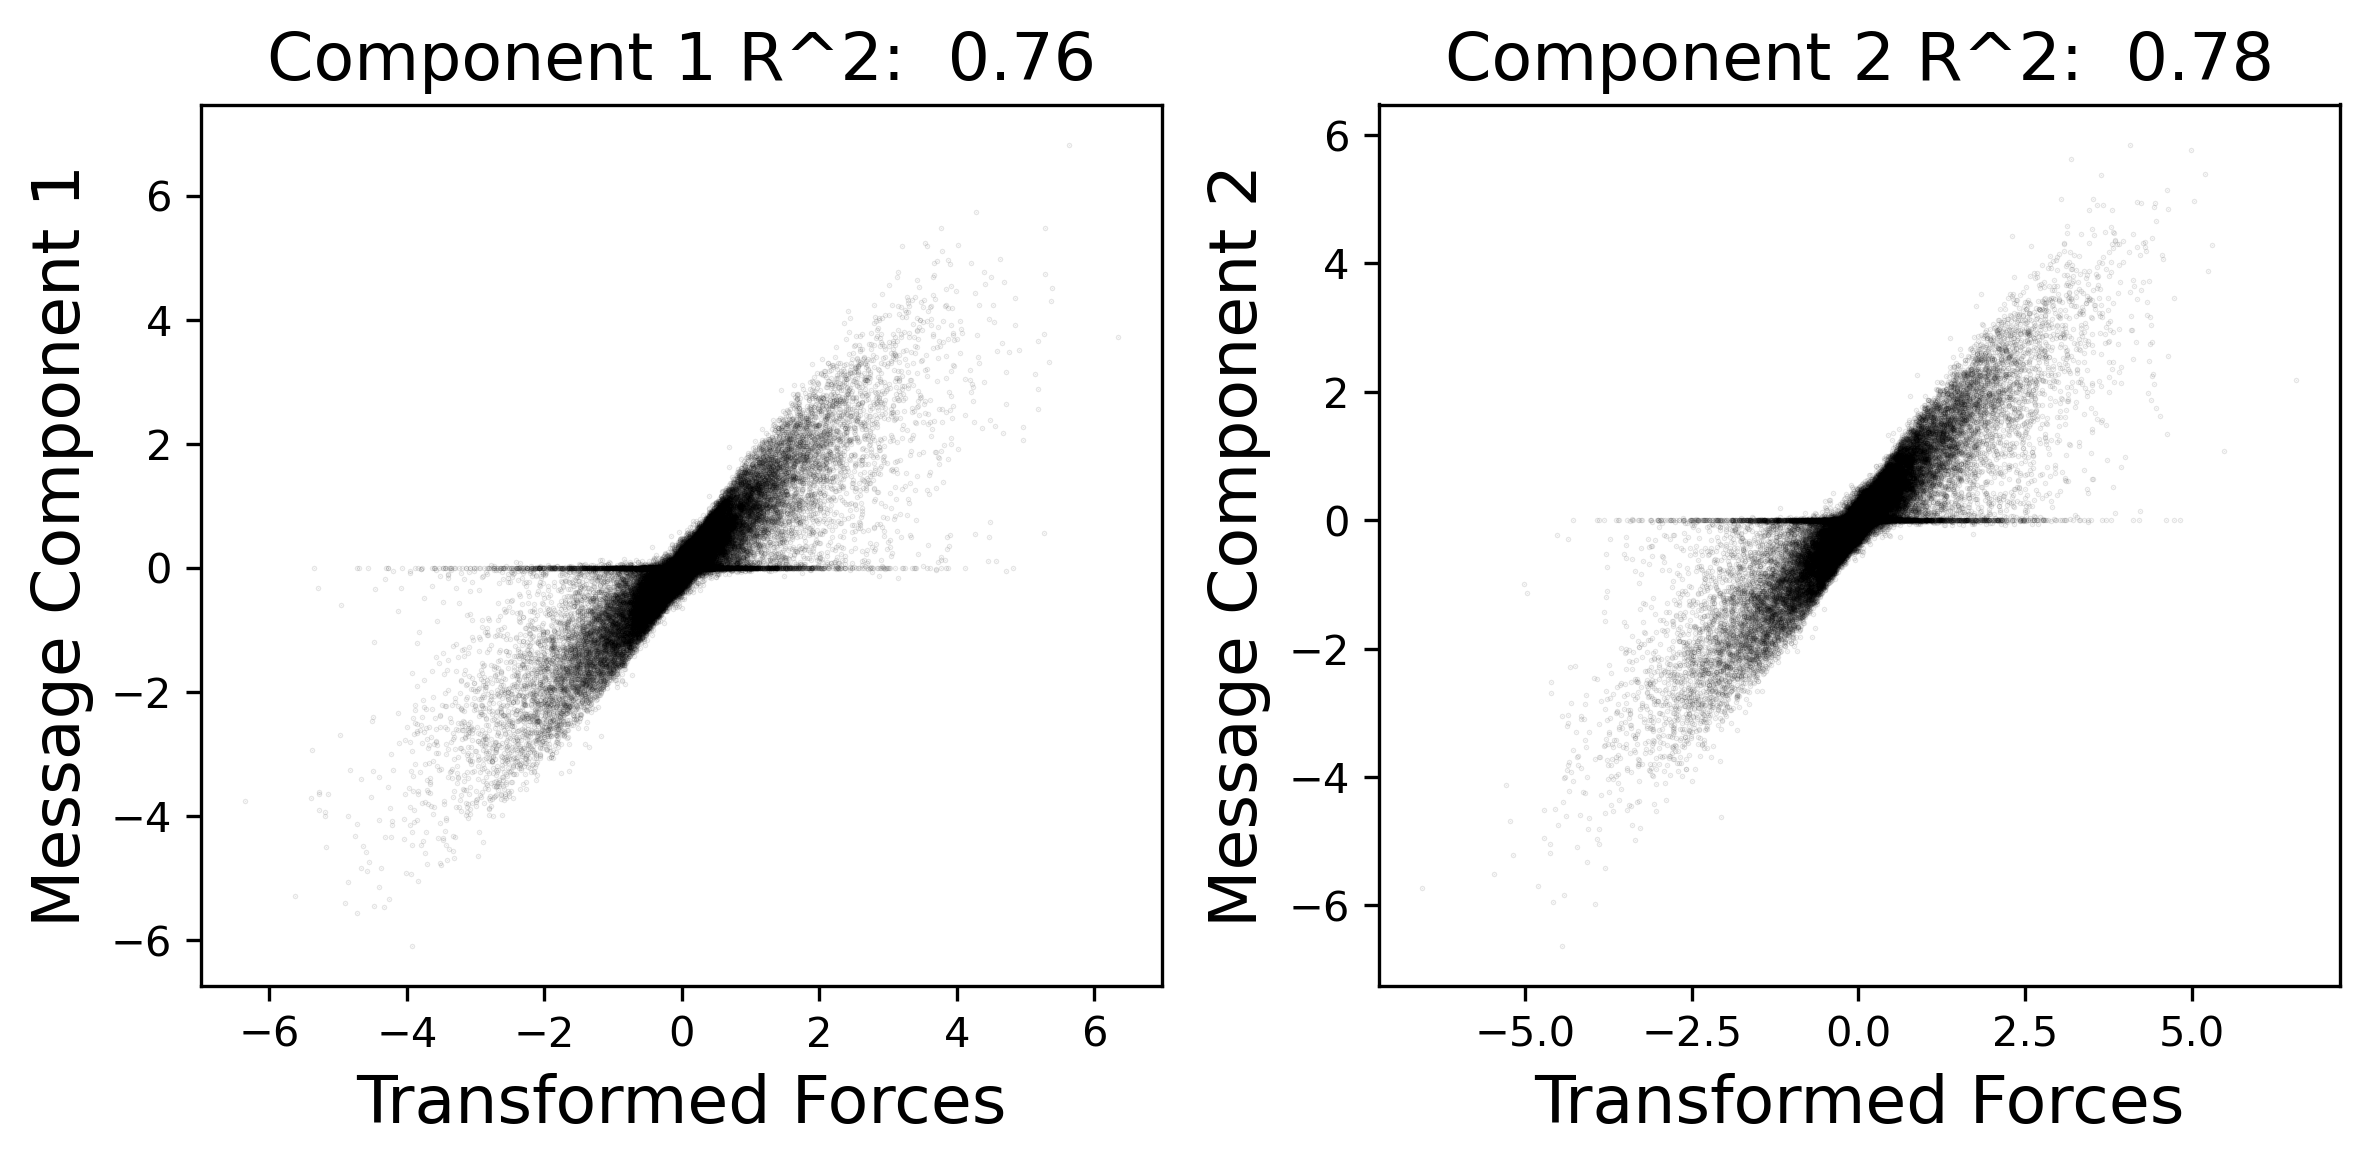
\includegraphics[width=\textwidth]{figs/spring_2d_kl_r2.png}
            \caption{Spring 2D, KL}
        \end{subfigure}
        \caption{Scatter plots of the edge message components against the linear transformation of the pairwise force for the different strategies of the spring 2D simulation.}
        \label{fig:scatter_plots}
    \end{figure}
    \subsection{Edge Message Sparsity}
    Next, to investigate the sparsity of the edge messages under the different training strategies, the percentage of total edge message variance across all components explained by the top $d$ components, where $d$ is the dimensionality of the problem, is calculated. The results are presented in Table \ref{tab:scarcity}. The KL and L$_1$ strategies consistently outperform the standard strategy. This suggests that the KL and L$_1$ strategies are more effective than the baseline at promoting sparsity in the edge messages. Note, the bottleneck strategy will always have, by definition, 100\% of the edge message variance explained by the top $d$ components.
    \begin{table}[H]
        \centering
        \begin{tabular}{lcccc}
        \hline
        Sim & Standard & Bottleneck & L$_1$ & KL \\
        \hline
        Charge-3 & 0.404 & 1.000 & 0.474 & 0.550 \\
        Charge-2 & 0.180 & 1.000 & 0.263 & 0.667 \\
        r$^{-2}$-3 & 0.583 & 1.000 & 0.795 & 0.925 \\
        r$^{-2}$-2 & 0.374 & 1.000 & 0.525 & 0.712 \\
        r$^{-1}$-3 & 0.877 & 1.000 & 0.743 & 0.719 \\
        r$^{-1}$-2 & 0.591 & 1.000 & 0.925 & 0.990 \\
        Spring-3 & 0.889 & 1.000 & 0.999  & 0.993 \\
        Spring-2 & 0.737 & 1.000 & 1.000 & 0.989 \\
        \hline
        \end{tabular}
        \caption{Fraction of total edge message variance across all components explained by the top $d$ components, where $d$ is the dimensionality of the problem.}
        \label{tab:scarcity}
    \end{table}

\subsection{Symbolic Reconstructions}
The next set of results relate to the symbolic distillation of the edge and node models. The edge and node models are distilled seperately using the method outlined. The edge model's distillation should yield an expression which is approximately analogous to a linear transformation of the true force, whereas the node model's distillation should yield an expression which resembles Newtons second law.
\begin{table}[H]
        \centering
        \begin{tabular}{lcccc}
        \hline
        Sim & Standard & Bottleneck & L$_1$ & KL \\
        \hline
        Charge-3 & \textbf{3/3} & \textbf{3/3} & 0/3 & 0/3 \\
        Charge-2 & 0/2 & \textbf{2/2} & 1/2 & 0/2 \\
        r$^{-2}$-3 & 1/3 & \textbf{3/3} & \textbf{3/3} & 0/3 \\
        r$^{-2}$-2 & 0/2 & \textbf{2/2} & 0/2 & 1/2 \\
        r$^{-1}$-3 & \textbf{3/3} & \textbf{3/3} & 2/3 & \textbf{3/3} \\
        r$^{-1}$-2 & 0/2 & \textbf{2/2} & \textbf{2/2} & \textbf{2/2} \\
        Spring-3 & 0/3 & 2/3 & 2/3  & 0/3 \\
        Spring-2 & 1/2 & \textbf{2/2} & \textbf{2/2} & 0/2 \\
        \hline
        \end{tabular}
        \caption{Successful reconstructions of the pairwise force (or acceleration) after symbolically regressing the edge model. Experiments where all components are successfully reconstructed are highlighted in bold.}
        \label{tab:sr_edge_model_table}
    \end{table}
From the results obtained, it is clear that the bottleneck strategy consistently outperforms the other strategies in the symbolic distillation of the edge model, the L$_1$ strategy is the next most successful, followed by the standard strategy and the KL strategy. The success of the standard strategy is suprising as in the original paper, it was not found to give any successful reconstructions.

\paragraph*{Example successful reconstructions} of recovering the pairwise force (or acceleration) after symbolically regressing the edge model.
    \begin{itemize}
        \item
        Spring 2d, L$_1$ (expect $\phi^{e}_i \approx \mathbf{a} \cdot (1-\frac{1}{r}) \mathbf{\Delta {r}} + b$):
        $$
        \phi^{e}_1 = (-0.291 + \frac{0.287}{r})(\Delta x - 0.986 \Delta y) + 0.00118
        $$
        \item 
        r$^{-1}$ 2d, KL (expect $\phi^{e}_i \approx \mathbf{a} \cdot \frac{m_1 m_2}{r^2} \mathbf{\Delta r} + b$):
        $$\phi^{e}_2 = -\frac{0.273m_2(\Delta x + \Delta y)}{r^2}$$
        \item 
        r$^{-2}$ 3d, bottleneck (expect $\phi^{e}_i \approx \mathbf{a} \cdot \frac{m_1 m_2}{r^3} \mathbf{\Delta r} + b$):
        $$\phi^{e}_3 = \frac{6.06m_2(-0.713\Delta x + \Delta y + 2.44\Delta z)}{r^3}$$
        \item 
        Charge 3d, standard (expect $\phi^{e}_i \approx \mathbf{a} \cdot \frac{q_1 q_2}{r^3} \mathbf{\Delta r} + b$. Note, because $q_1, q_2 \in \{-1, 1\}$, $q_1 \times q_2 \equiv \frac{q_1}{q_2} \equiv \frac{q_2}{q_1}$):
        $$\phi^{e}_1 = = -\frac{39.3q_2(0.273\Delta x + \Delta y)}{ q_1 m_1r^3}$$
    \end{itemize}
    Here, $\mathbf{a} = (a_1, a_2)$ and $b$ are constants, $\mathbf{\Delta r} = (\Delta x, \Delta y, \Delta z)$ represents the displacement vector, $q_1, q_2$ are the charges and $m_1, m_2$ are the masses. $\phi^{e}_i$ is the $i$th most significant component of the edge message, reflecting the interaction from body 2 to body 1. Note how the reconstruction for the shown spring 2d experiment is a linear transformation of the true pairwise force whereas the other expressions have divided through by the mass of the receiving particle, $m_1$, and thus represent the acceleration.

    The results of the symbolic distillation of the node model are presented in Table \ref{tab:sr_edge_model_table}. Here, the standard strategy yields the best results, followed by bottleneck, L$_1$  and finally, the KL strategy.
    \begin{table}[H]
        \centering
        \begin{tabular}{lcccc}
        \hline
        Sim & Standard & Bottleneck & L$_1$ & KL \\
        \hline
        Charge-3 & \textbf{3/3} & 0/3 & 0/3 & \textbf{3/3} \\
        Charge-2 & 0/2 & 0/2 & 0/2 & 0/2 \\
        r$^{-2}$-3 & \textbf{3/3} & \textbf{3/3} & \textbf{3/3} & 0/3 \\
        r$^{-2}$-2 & 0/2 & \textbf{2/2} & 0/2 & 0/2 \\
        r$^{-1}$-3 & \textbf{3/3} & \textbf{3/3} & 2/3 & 0/3 \\
        r$^{-1}$-2 & \textbf{2/2} & \textbf{2/2} & \textbf{2/2} & 0/2 \\
        Spring-3 & \textbf{3/3} & \textbf{3/3} & \textbf{3/3}  & 0/3 \\
        Spring-2 & \textbf{2/2} & \textbf{2/2} & \textbf{2/2} & 0/2 \\
        \hline
        \end{tabular}
        \caption{Successful reconstructions of the Newton's 2nd law after symbolically regressing the node model. Experiments where all components are successfully reconstructed are highlighted in bold.}
        \label{tab:sr_edge_model_table}
    \end{table}


\paragraph*{Example successful reconstructions} of recovering Newtons 2nd law after symbolically regressing the node model (expect $\phi^{v}_i \approx \frac{\mathbf{a} \cdot \mathbf{\bar{e}} + b}{m_1}$, where $\mathbf{\bar{e}}$ is the aggregated edge message and $m_1$ is the mass of the receiving particle).
\begin{itemize}
        \item
        Spring 2d, L$_1$:
        $$
        \phi^{v}_1 = \frac{0.199\bar{e_1} - 0.509\bar{e_2} + 0.0316}{m_1}$$
        \item
        r$^{-1}$ 3d, standard:
        $$
        \phi^{v}_2 = -0.00317\bar{e_3} - 0.00379\bar{e_1} - 0.00253\bar{e_2} + 0.00396
        $$
        \item
        r$^{-2}$ 2d, bottleneck:
        $$
        \phi^{v}_1 = 7.76\bar{e_1} - \bar{e_2}
        $$
        \item
        Charge 3d, KL:
        $$
        \phi^{v}_2 = \frac{0.147(\bar{e_1} + \bar{e_2})}{m_1}
        $$
    \end{itemize}

    In some cases, the node model is a simple linear transform of the aggregated edge messages, this occurs when the edge model learns the pairwise acceleration, so the node model just acts as a sum over the individual accelerations to return the net acceleration. In other cases, like the charge 3d KL experiment and the spring 2d L$_1$ experiment, the node model explicitly learns the division by the mass of the receiving particle, $m_1$, to convert the force to an acceleration.

    Finally, the performance of the symbolic models are compared to the neural network models in Table \ref{tab:sr_vs_nn_table}. This is done choosing experiments where all components of the edge and node model outputs could be successfully reconstructed and comparing the MAE and standard deviation on the test set from the symbolic model against the best performing neural network for that simulation. The neural network generally outperforms the symbolic model. It is worth noting that the constants in the symbolic model were not refit to the data as suggested in the original paper. 
    \begin{table}[H]
        \centering
        \begin{tabular}{lcccc}
        \hline
        Sim & Symbolic & Neural Net \\
        \hline
        Charge-3 & 2.775 $\pm$ 0.305 & \textbf{0.110} $\pm$ 0.015 \\
        r$^{-2}$-3 & 3.225 $\pm$ 1.084 & \textbf{0.518} $\pm$ 0.998\\
        r$^{-2}$-2 & 1.956 $\pm$ 1.110 & \textbf{0.450} $\pm$ 0.142 \\
        r$^{-1}$-3 & 0.161 $\pm$ 0.027 &\textbf{0.0261} $\pm$ 0.003 \\
        r$^{-1}$-2 & 0.0290 $\pm$ 0.006 & \textbf{0.0238} $\pm$ 0.005 \\
        Spring-2 & 0.0234 $\pm$ 0.002 &\textbf{0.0182} $\pm$ 0.001 \\
        \hline
        \end{tabular}
        \caption{Symbolic model versus neural network, performance compared by MAE on the test set, presented as mean $\pm$ standard deviation. The best values across different models are shown in bold.}
        \label{tab:sr_vs_nn_table}
    \end{table}
\section{Discussion}
In this section the results are discussed, both in a standalone manner and in the context of the original paper's results. 
\subsection{Model Performance}
% The difficulty increasing wrt to the inverse force
To understand the results, it is first imperative to understand that the force laws simulated in this report vary in complexity. This complexity can be understood in terms of dependencies on the distance \( r \). Specifically, the spring force is linearly proportional to \( r \) whereas the orbital force laws follow \( r^{-1} \) and \( r^{-2} \) dependencies. The electrostatic force also follows a \( r^{-2} \) dependency. This leads to significant differences in how data varies across simulations, as detailed by the standard deviation of the acceleration labels in the training set (Table \ref{tab:std_table}).
\begin{table}[H]
    \centering
    \begin{tabular}{lcc}
    \hline
    Sim & Standard Deviation \\
    \hline
    Charge-3 & 14 \\
    Charge-2 & 75 \\
    r$^{-2}$-3 & 31 \\
    r$^{-2}$-2 & 150 \\
    r$^{-1}$-3 & 5.3 \\
    r$^{-1}$-2 & 7.6 \\
    Spring-3 & 15 \\
    Spring-2 & 6.8 \\
    \hline
    \end{tabular}
    \caption{Standard deviation of the acceleration labels in the training set for the different simulations.}
    \label{tab:std_table}
\end{table}
Table \ref{tab:std_table_2} ranks the networks by the standard deviation of the accelerations in their training data and their MAE on the test set. The results show how the standard deviation of the accelerations in the training set can predict the performance of the model on the test set. Which makes intuitive sense, it is harder for the model to learn robust features if the data varies over too large a scale. Further, it explains why the performance on the 2D data for a given force law is worse than the 3D data, in all cases except spring where the situation is reversed due to it being proportional to a positive power of $r$. Due to the higher dimensionality of the problem, there is more 'space' so there is a smaller chance any pair of particles get too close to each other and the acceleration blows up. This is why the models trained on 3D data perform better than those trained on 2D data. For the spring experiment, the larger distances between particles in 3D means that the accelerations will be larger and hence why for spring, the 2D simulation performs better. It is worth noting that the MAE values presented in the original report, shown in Table \ref{tab:mae_table_original} are also consistent with this point. The main point of contention is how the original paper frames the results as the L$_1$ strategy being the best when both the reproduction and the original results show how the results are very close. Indeed, in this report the 
bottleneck strategy was found to be the best in five out of eight simulations by a slim margin, however factoring in the standard deviations in the MAE scores, one can see how the strategies are very close in performance. As such, there is no clear dominant strategy, only a clear worst one in the KL strategy.
% Discuss the results of the MAE and std.
\begin{table}[H]
    \centering
    \begin{tabular}{lccc}
    \toprule
    Performance & Training Label Std. Dev. & Test Set MAE\\
    \midrule
    1 (\textbf{Best}) & spring-2 & spring-2 \\
    2& r$^{-1}$-3 & r$^{-1}$-2  \\
    3& r$^{-1}$-2 & r$^{-1}$-3 \\
    4& spring-3 & spring-3\\
    5& charge-3 & charge-3\\
    6& r$^{-2}$-3 & r$^{-2}$-3\\
    7& charge-2 & r$^{-2}$-2\\
    8 (\textbf{Worst})& r$^{-2}$-2 & charge-2\\
    \bottomrule
    \end{tabular}
    \caption{Comparative analysis of model performance, correlating the standard deviation of the acceleration labels in the training set with the mean absolute error (MAE) on the test set.}
    \label{tab:std_table_2}
\end{table}
Further, the original papers MAE's are consistently higher, despite training for twice as long on twice as much data. At its extreme, the difference between the MAE presented in this report versus the originals was 49, compared to 0.462 for the standard charge 2d model. This likely means that the original data contained more extreme values, otherwise such a result is unexplainable. This motivates the importance of the pruning preprocessing step, which was not used in the original paper, however was essential in this reproduction. Without pruning the data, the KL training strategy was not found to be stable, with it's gradients exploding shortly into training, giving rise to nans in the loss. It is worth noting that the pruning is not the only solution to handling the large accelerations. These outliers were only an issue for the KL training strategy, where the predicted log variance terms would blow up after exponentiating them to compute the loss. One solution would be to squash the log variance term, alternatively the epsilon term added to the distance could be increased when generating the data. It would be interesting to see if the recovered symbolic expressions would then learn the larger epsilon term.
\subsection{Edge Message $R^2$}
\begin{figure}[H]
    \centering
    \begin{subfigure}{0.45\textwidth}
        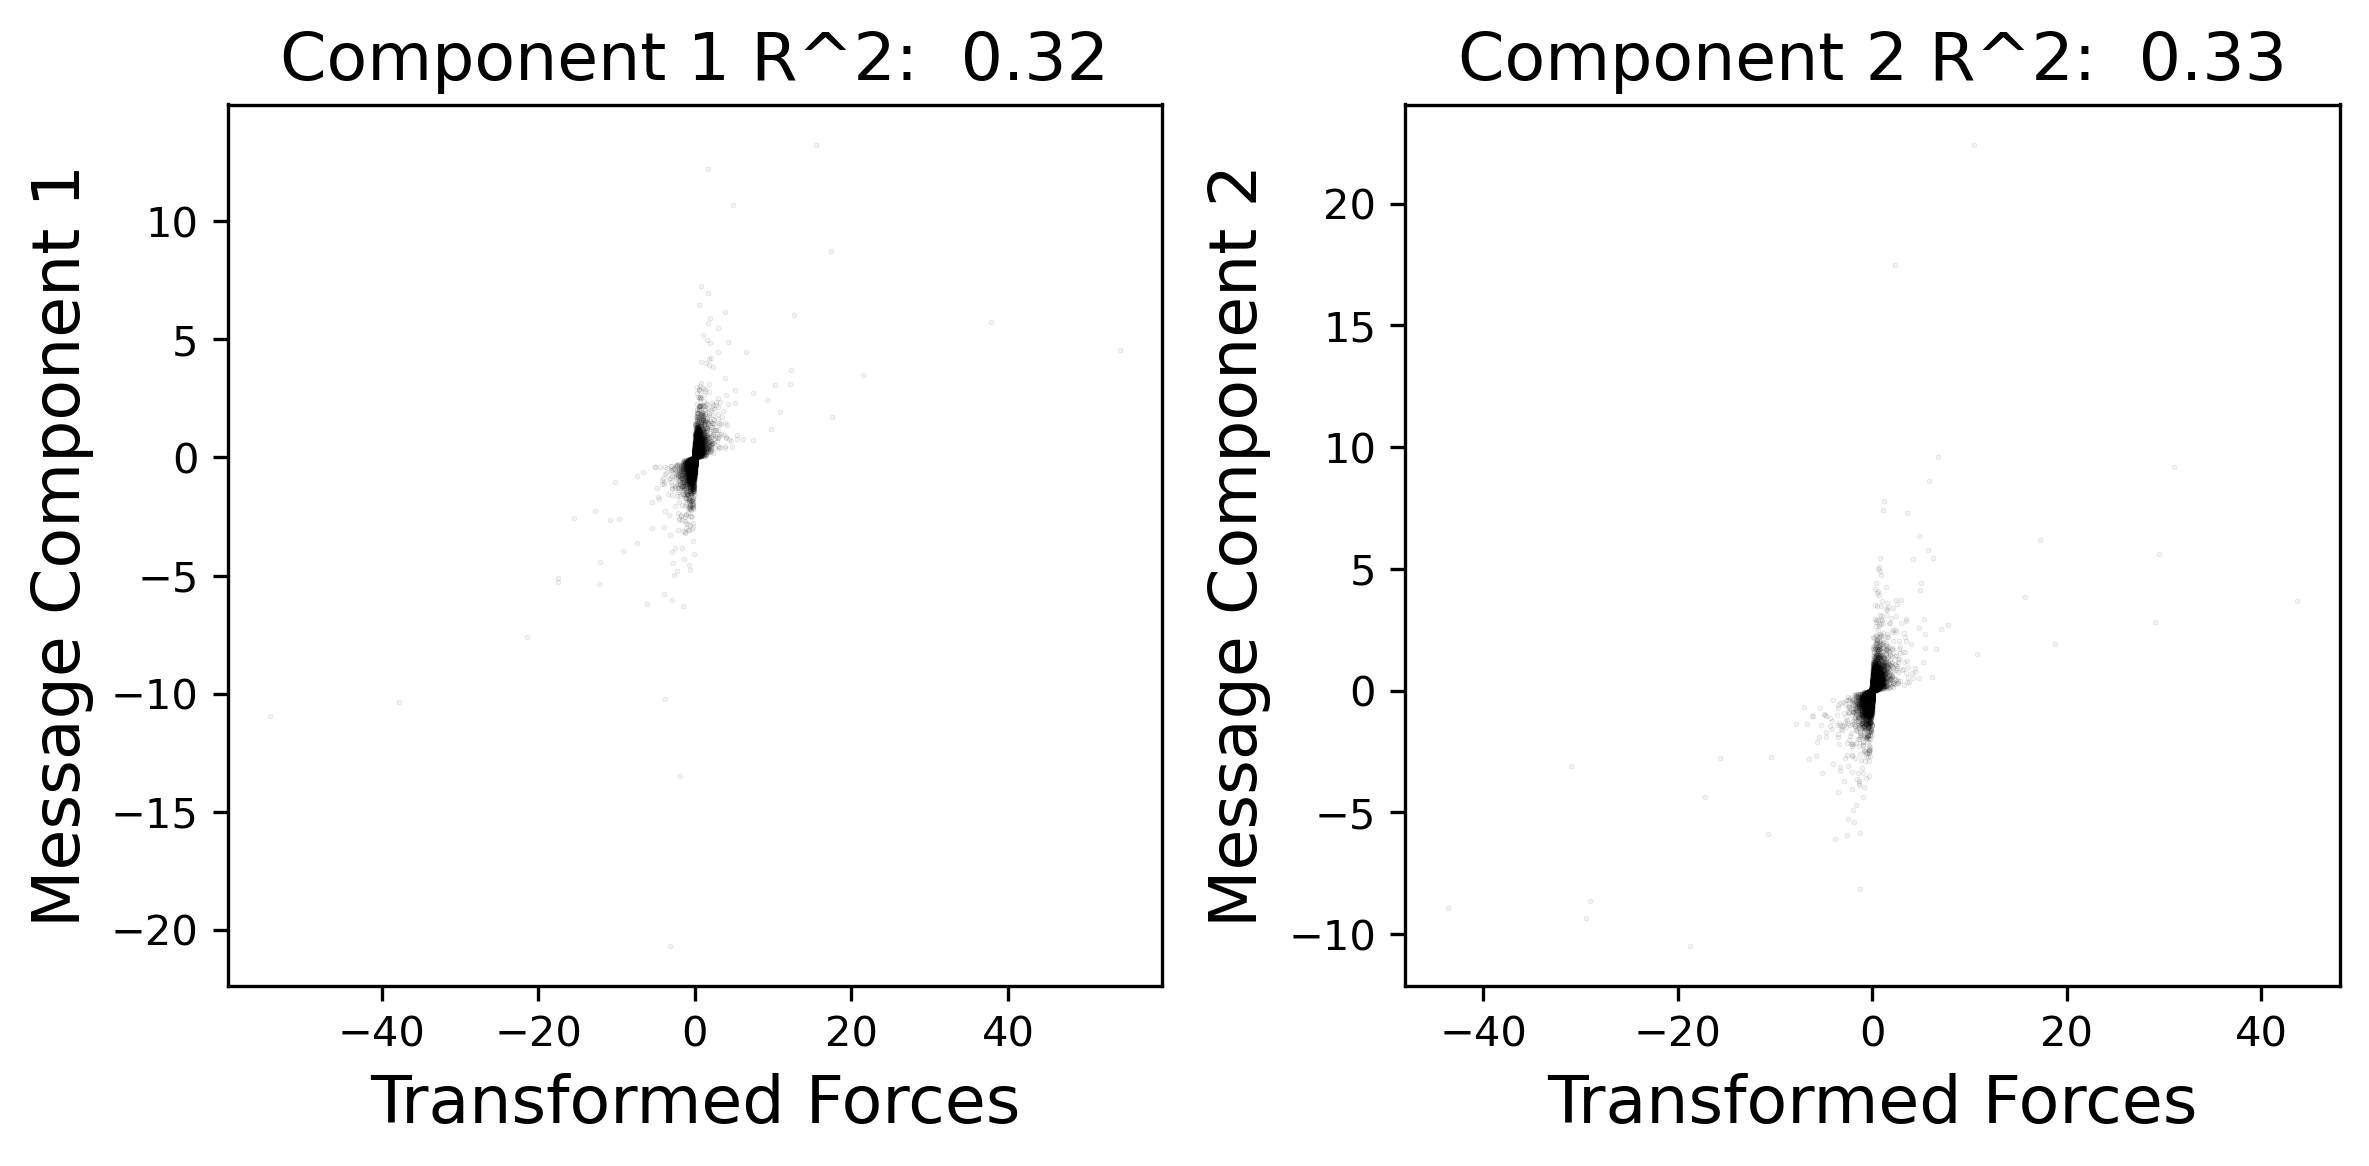
\includegraphics[width=\textwidth]{figs/r1_2d_force_r2.png}
        \caption{}
    \end{subfigure}
    \begin{subfigure}{0.45\textwidth}
        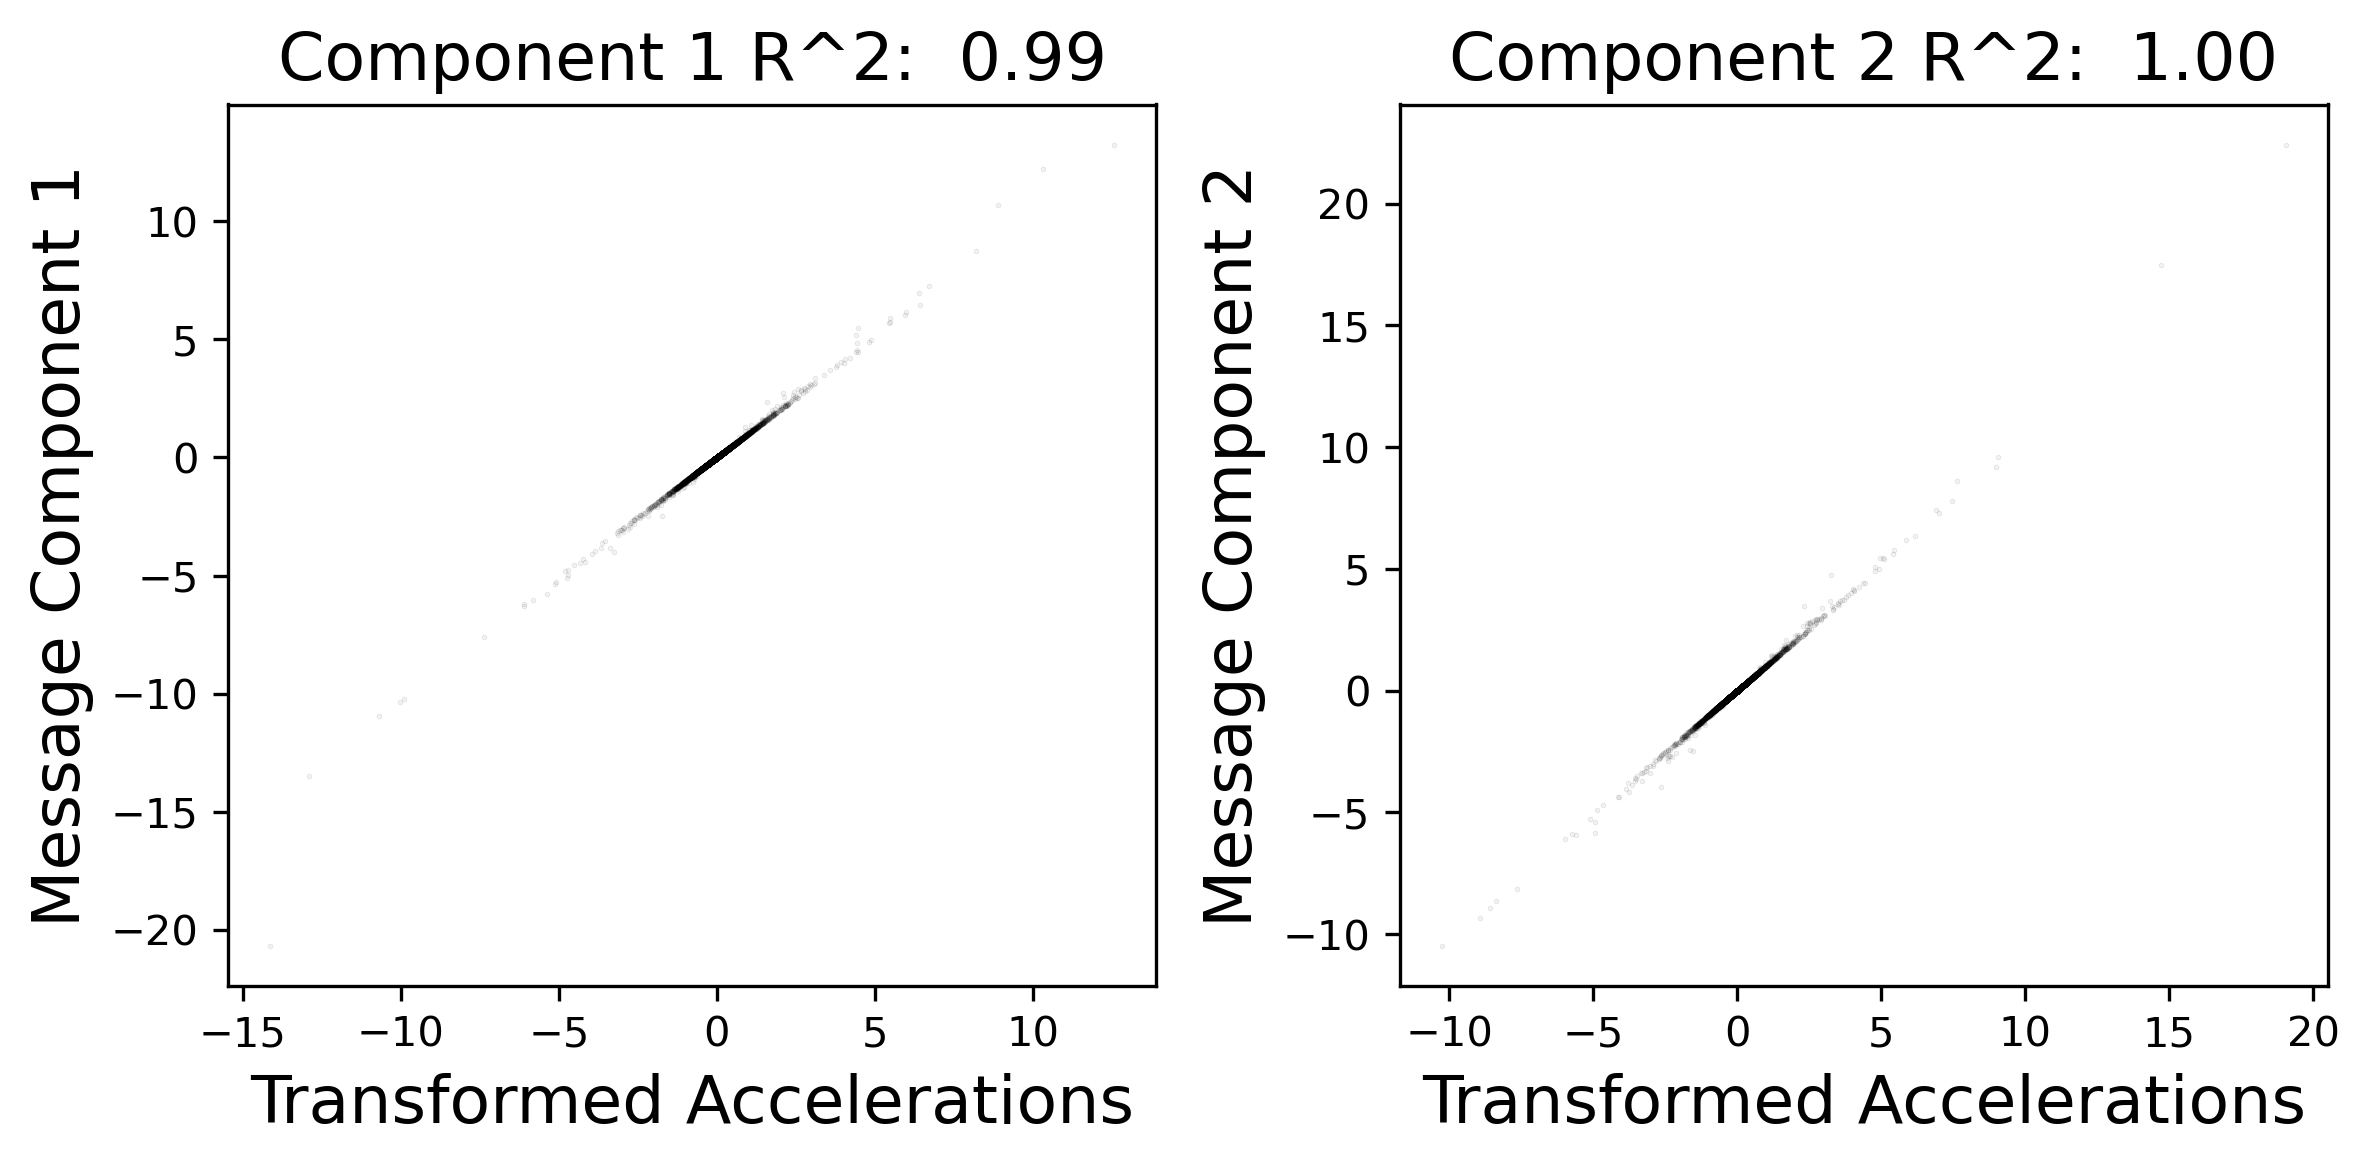
\includegraphics[width=\textwidth]{figs/r1_2d_accel_r2.png}
        \caption{}
    \end{subfigure}
    \caption{Comparison of scatter plots of the edge message components for $r^{-1}$ 2D, L1 experiment against a linear transformation of the a)  pairwise force b) pairwise acceleration.}
    \label{fig:scatter_plots}
\end{figure}
% Compare plot when
The next set of results to discuss are those presented in Table \ref{tab:R2}. These show the $R^2$ values of the edge message components against the transformation of the true force or acceleration. It is important to highlight that the edge model may sometimes learn pairwise acceleration directly, rather than pairwise force. This was also evident in the original paper, where the $1/r^2$ bottleneck experiment was shown to give the pairwise acceleration, however, the implications of this were not explored. Table \ref{tab:R2} and Figure \ref{fig:scatter_plots} explicitly demonstrate that $R^2$ values can be misleading if both pairwise force and acceleration are not separately considered. For clarity, two $R^2$ values are reported: one for pairwise force and one for pairwise acceleration. Generally, when one value is low, the other tends to be high, suggesting that the model captures relevant physical interactions rather than failing to represent the data appropriately. Contrary to the original paper, which suggests that the standard strategy yields almost zero $R^2$ values in all cases, findings in this report do not support this claim. The observed differences likely stem from variations in the datasets used. To further investigate this, multiple datasets could be generated using different seeds, and the analysis could be repeated.


\subsection{Edge Message Sparsity}
% Sparsity in edge message not signficantly correlated with higher chance of symbolic reconstrucion, eg KL having sparser messages than L1 but being worse in the symbolic reconstruction. 
The next set of results to be discussed are those presented in the Table \ref{tab:scarcity}, showing the fraction of the total variance captured by the $d$ most significant components in the edge message, where $d$ is the dimensionality of the problem. The general argument presented in the original paper was that promoting sparsity in the edge message would lead to a greater probability of successful symbolic reconstructions. However, the findings for KL training strategy provide an interesting example where the edge messages were often found to be sparser than those coming from networks trained under the L$_{1}$ strategy, however it was the strategy which had the lowest number of successful symbolic reconstructions. It is possible that the inductive bias placed on the model by the KL strategy was not appropriate for the task at hand. Alternatively, it may be the case that weight of the regularisation term was simply too large. The high MAE values over the test set also indicate that the model may have over prioritised sparsity in the edge message. Further, it is interesting to note that the opposite case is also true, where a lack of sparsity in the edge messages does not necessarily mean that the symbolic regression will fail. The charge 3D standard experiment is a good example of this, where the edge messages were not particularly sparse, with the top 3 components only capturing 40\% of the total variance, however all components were successfully reconstructed. 
\subsection{Symbolic Reconstructions}
% Discuss the edge reconstruction results - bottleneck wins, followed by l1, then standard and KL. 
Finally, the symbolic reconstructions are discussed. First the edge model's reconstructions are considered. It is no suprise that the bottleneck strategy is the most successful, as it places the strongest inductive bias, explicitly constraining the message latent space to be of the correct dimensionality. However, what is suprising is that the standard model performed better than in the original paper, which found that no model trained under the standard strategy could yield a successful reconstruction. Here, it was found that the standard strategy was able to give some successful reconstructions, despite not having any explicit strategy to promote sparsity in the edge messages. Which suggests that the inductive biases of a message-passing neural network, which calculates acceleration from aggregated messages, might be better than originally presented. This conclusion is supported by the $R^2$ values observed, which were comparable to those obtained under strategies explicitly encouraging sparsity.

% Explain why R2 is more useful metric to determine which experiments were successful.
To frame this discussion, it is important to understand the relevance of the $R^2$ Table \ref{tab:R2}. Since the true underlying force law is known and can be expressed perfectly in terms of summed messages, it is known that the symbolic model for the edge message will be a linear transformation of the true force. As such an $R^2$ value close to 1 is a sufficient condition for one to conclude that the model can be expressed as a symbolic equation. Therefore, the $R^2$ values can be used as a proxy to determine which training strategies were successful, which show that the standard, bottleneck and L1 strategies should all have more successful reconstructions than have been reported. The issue with retrieving a symbolic model is that the search space is vast, despite using a subset of the operators considered in the original paper to reduce the search space. For example, the spring 3d bottleneck provides a good example of this point. Since it had an $R^2$ value close to 1, it was assumed that the model had learned an appropriate representation of the pairwise force. However, the symbolic search was unable to find any successful reconstructions in the first attempt. It took several more attempts before a search yielded components that were close to the true pairwise force. Other experiments such as the spring 2D, spring 3D and $r^-1$ 2D and standard experiments all have $R^2$ values close to 1, however the single search performed was unable to find a successful reconstruction. It is very likely that if a longer search was done, as was the case for the spring 3D bottleneck experiment, a successful reconstruction would have been found. Therefore, the reconstructions presented should not be used as an absolute measure of the success of the training strategy, but rather an indication of what is possible to recover with a quick search. It is also important to note that while it is not strictly necessary that the experiment have a high $R^2$ value in order for symbolic regression to be successful, it is also the case that one would expect the $R^2$ value to indicate moderate correlation if the symbolic regression was successful. However, the original paper presents two odd cases, where for the KL strategy, the spring and $r^{-1}$ 3D experiments had very low $R^2$ values of was 0.214 and 0.332, respectively, yet both were stated to give successful reconstructions. Such a result is quite rare and would be interesting to investigate further. 
% Discuss the results of the node model - l1  wins, followed by standard, bottleneck and KL.

Next the node model results are discussed. The results show that the standard, bottleneck and L1 and standard strategies all perform well. It is interesting to note how much better the node reconstructions were for the standard strategy compared to the edge reconstructions. This is likely because of the fact that neural networks like to learn simple identity functions where possible. In this case, the architecture of the GNN allows for the node model to act as a simple sum function which may explain the higher success rate of the node reconstructions compared to the edge reconstructions. Future work could include creating $R^2$ tables for the node model to better understand if reconstructions were missed as discussed earlier or if the experiments were truly unsuccessful. This could be done by finding the correlation between the node model outputs and a linear transform of the aggregated edge message and node features in the same way as was done for the edge model.

It is worth noting that sometimes the correct reconstruction was not the best, however were excluded, to strictly adhere to the selection criteria outlined. In practice this would be relaxed. Further, some reconstructions were very close to the expected result, examples of close reconstructions are given in the appendix. 

The final set of results to discuss are those from comparing the symbolic model's performance to the trained networks. The results show that the symbolic model generally performs worse than the corresponding neural networks. This is likely to be because the constants in the symbolic model were not refit to the data as suggested in the original paper. Given that there is no noise in the dataset, one would expect the symbolic model to perform at least as well as the neural network, if not better. It is likely performing worse due to the accumulated approximation error from the multiple levels of function fitting. It would be interesting to see how the symbolic model would perform if the constants were refit to the data.

\subsection{Future work}
    % Dataset reproduction being very hard.
    There are two primary means by which this reproduction study could be further improved. The first being to repeat the analysis for different random seeds and seeing if the different sets of trained models are consistent with the results presented in this report. This would help give an understanding of what is natural variation in the results due to the stochastic nature of the training process versus what is a systematic discrepancy between the reproduced study and the original findings. Such an approach would solidify the conclusions drawn and provide a clearer comparison between the varying strategies employed for both the edge and node models.

    The second means by which this reproduction study could be further improved is to investigate the effect incorporating more inductive biases and seeing if the trained models are easier to distill as would be expected. A natural bias to add to the model would be to include Newtons third law, through introducing a penalty to the loss term that enforces the sum of $\mathbf{\phi^{e}(x_i, x_j)} + \mathbf{\phi^e(x_j,x_i)} = \textbf{0}$.

% \section{ Reproducibility}
% This section addresses the reproducibility aspect of this work. There are 3 sources of randomness at play which affect the ability to reproduce the results. 
% \subsection{Dataset Reproducability}
% The first challenge reproducing the results of the original paper was in reproducing the datasets. The original paper did provide the code used to generate the datasets, however did not indicate which seeds were used. However, even if this was declared, the datasets would still be difficult to reproduce, due to the differences in hardware. $N$ body simulations, where $N > 2$, are famously chaotic systems. This means that small changes in the initial conditions can lead to vastly different outcomes. Or in this case, small numerical fluctuations introduced through the hardware specific optimisations that the \texttt{jax} package uses can lead to drastically different trajectories. To demonstrate this point, two datasets are generated following the $r^{-1}$ force law, for 4 bodies in 2 dimensions. The datasets describe 10000 simulations of 30 time steps each. The same random seed was used to generate both datasets, however the datasets were generated on different machines, the first was generated locally on a laptop using macOS and the second was generated through a system running linux. The Kologorov-Smirnov test was used to compare the distributions of the particle's $x$ coordinate as a function of time across all simulations. The results are shown in Figure \ref{fig:ks_test}. The figure shows how the p value rapidly decreases as the time step increases, indicating that the distributions quickly diverge. 

% \begin{figure}[H]
%     \centering
%     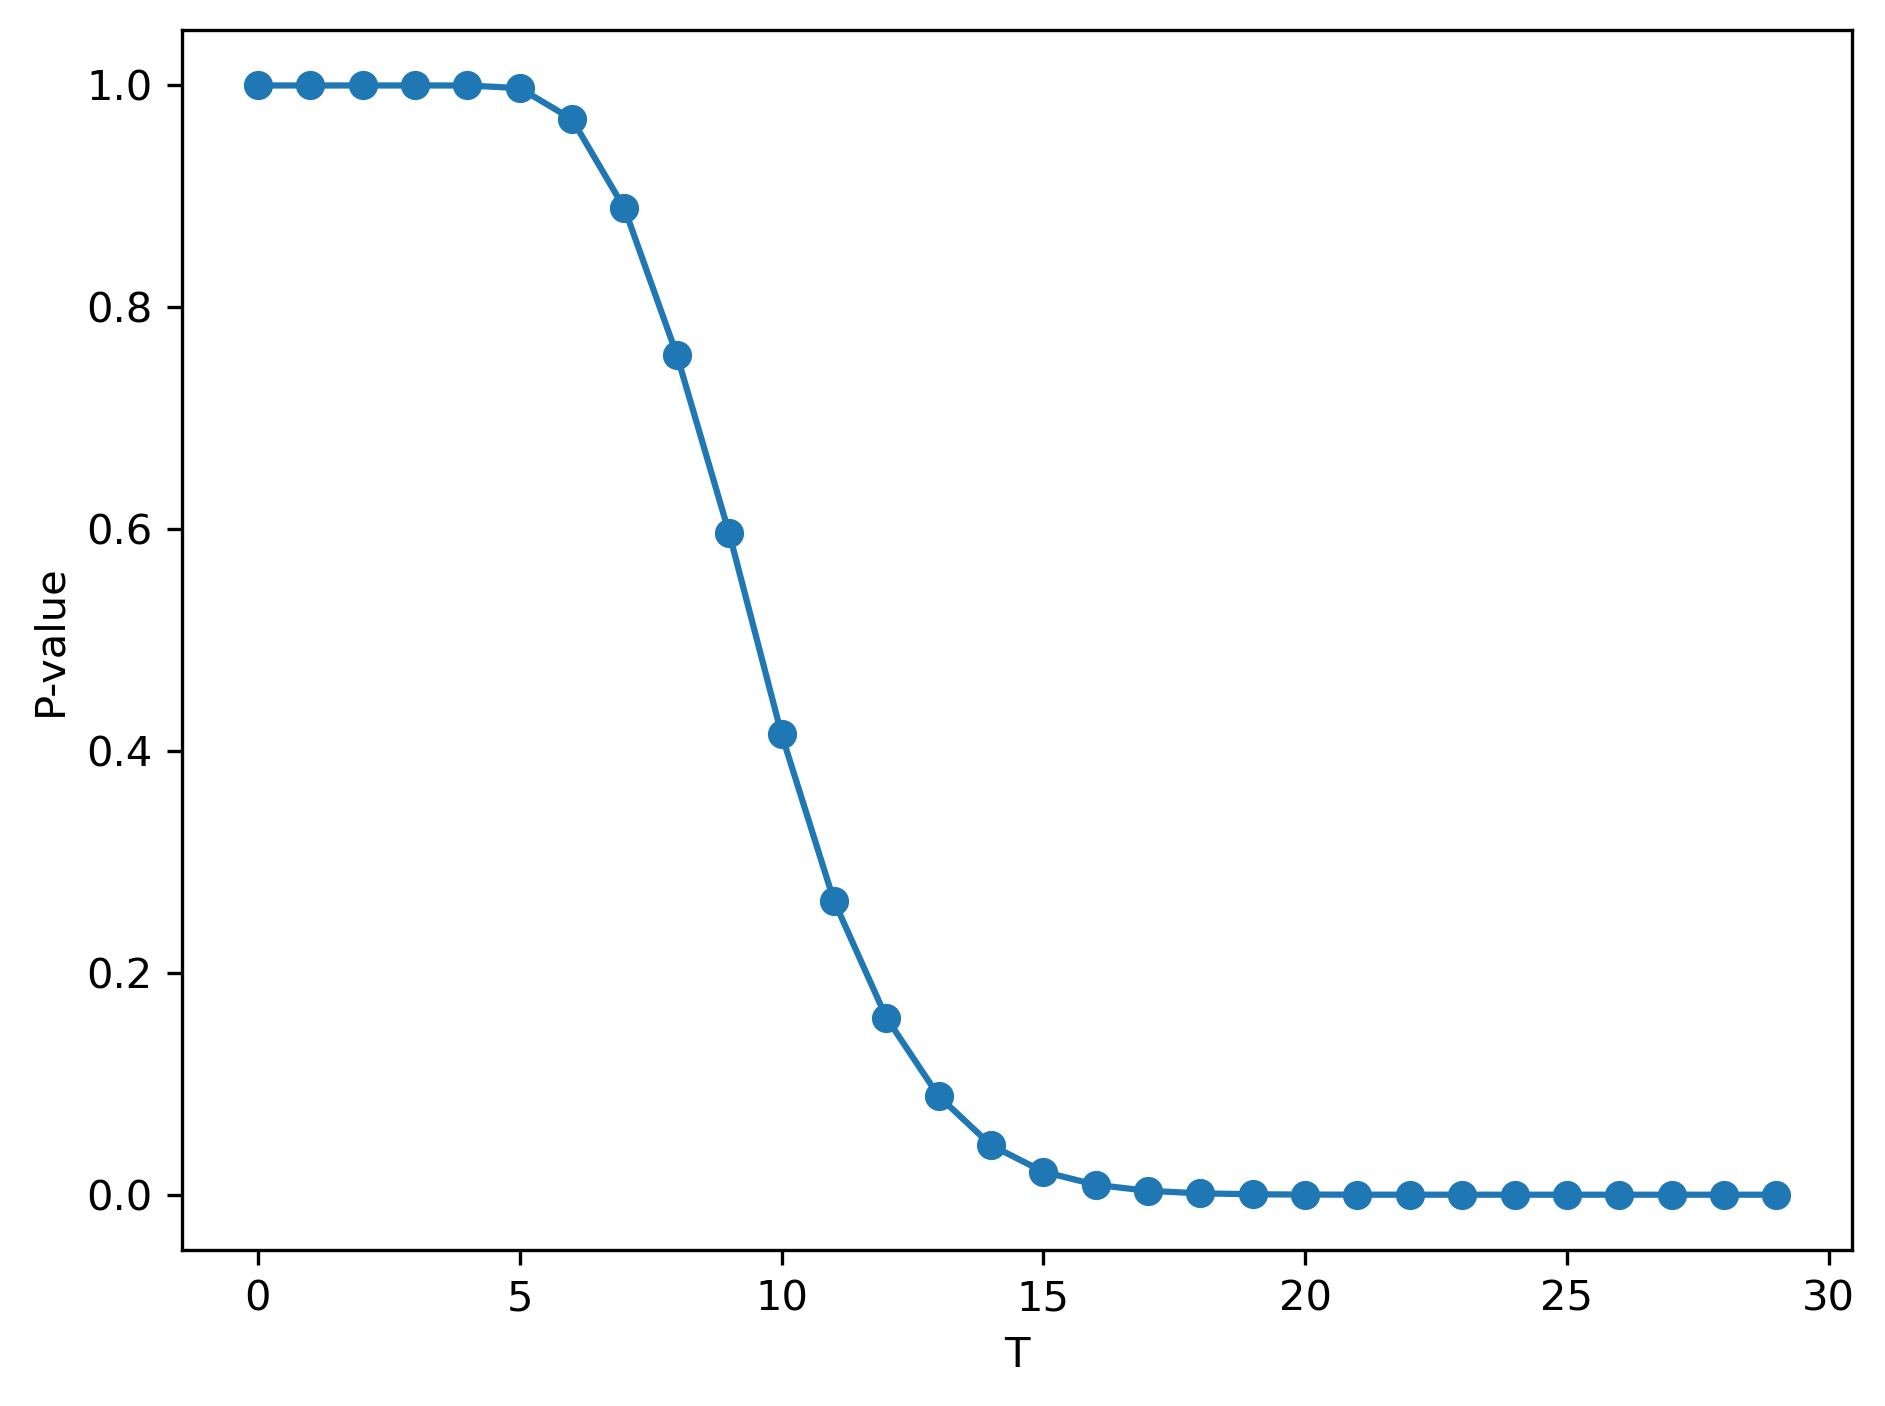
\includegraphics[width=0.5\textwidth]{figs/ks_test.png}
%     \caption{Kologorov-Smirnov test comparing the distributions of the particles $x$ coordinate as a function of time, $T$ across an interacting particle dataset. The test was performed on two datasets generated using the same package versions and random seeds but on two different machines.}
%     \label{fig:ks_test}
% \end{figure}
% Thus, to address this issue, the datasets were generated using a docker container. This ensures a standardised environment in which to generate the datasets in a reproducible manner. Further, future work could instead incorporate datasets which use more simulations that are each evolved for fewer number of time steps which would help limit any error introduced by the chaotic nature of the system. Alternatively, the datasets could be hosted on a cloud service, such as AWS S3, which would circumvent the need to generate the datasets and guarentee that everyone is using the same data.

% \subsection{Model Reproducability}
% Next, even if the datasets can be perfectly reproduced, there are still stochastic elements in the training process which can affect the results. To resolve this, a random seed was used to make training deterministic and see the initial model weights are also saved during training. These can be made available upon request. Further, the code base was designed to give reproducible results. Conda was used to standardise the environment and configuration files used to run the experiments were stored in the git repository under \texttt{configs/train\_configs}. Every train job is automatically logged to wandb. The train config is also saved to the output directory of the train job with the current git commit hash. These configs and the trained models can be made available upon request, they have not been included in the git repository due to their size. Steps to reproduce the training process are detailed in the \texttt{README.md} file.

% \subsection{Symbolic Regression Reproducbility}
% Lastly, the symbolic regression process is also stochastic. The search space is vast and thus in order to get reproducible results, a random state was set. Further, the hyperparameters of the \texttt{PySRRegressor} were also made clear in the method section.

% % 3 sources of randomness - the dataset , model initialisation, optimisation / training, symbolic search. How to standardise each one in the future.

% % Dockerisation, conda, git, readme, etc.

\section{Conclusion}
This report has presented the results of a reproduction study of the paper "Discovering Symbolic Models using Deep Learning with Inductive Biases". Here a subset of the experiments introduced in the original paper were investigated. This report managed to find the same overall trends in the MAE values as the original paper. Symbolic reconstructions of the edge and node models were successfully found. With the bottleneck and L1 training strategies being the most successful in yielding the most reconstructions of the true force law as reported by the original paper. However, the standard strategy was found to be far more successful in learning a compact latent space than was suggested by the original paper. Thus, the main claim of the original paper, that symbolic regression can be used to distill the learned models of neural networks trained using appropriate inductive biases, was found to be true. 
%     Talk about perhaps the more sensible thing would be to distill one at a time in accordance with the framework.
%     Effect of training for fewer epochs
%     Discuss challenges reproducing the results of the paper.
%     Discuss how the code base is designed to give reproduible results
%     Dataset storage.
%     Dataset seed and local environment differences.
%     Try to generate the dataset from a docker container to standardise the environment.
%     Config files git commits, wandb
%     Future work, squash velocity, use a larger eps and see if the model can learn this, squash the log var. For data pre processing 
%     Preprocessing not in paper but got nans in kl otherwise
%     Explore purely velocity based pre pru
%     , NL3, enforcing correctness of dimensional units.
%     Discussion point - stronger L1 or an L1 scheduler type thing.
%     Could make the data more reproducable by fewer time steps and more simulations
    
\section{Appendix}
\subsection{Failed Symbolic Reconstructions}
\paragraph*{Example of some failed edge reconstructions:}
\begin{itemize}
    \item 

    Spring 2D, KL (clearly wrong):
    $$
    \phi^{e}_2 = \frac{\Delta x + \Delta y}{-r + m_1 ( 0.647 - m_1)}
    $$
    \item
    Charge 2D, L$_1$ (almost correct):
    $$
    \phi^{e}_2 = \frac{0.351\Delta y q_2}{r^2(r+0.169m_1)}
    $$
    \item
    $r^{-2}$ 3D, standard (almost correct):
    $$
    \phi^{e}_1 = \frac{8.43m_2(0.26+\frac{\Delta x - \Delta y + 3.52\Delta z}{r})}{r^2}
    $$
\end{itemize}
\paragraph{Example of some failed node reconstructions:}
\begin{itemize}
    \item 
    Charge 3D, KL (clearly wrong):
    $$
    \phi^{v}_3 = \bar{e_1}\bar{e_2}^2
    $$
    \item
    Charge 3D, bottleneck (almost correct):
    $$
    \phi^{v}_1 = (0.153 + \frac{0.171}{m_1})(\bar{e_2} + \bar{e_1} + 1.11)
    $$
    \item
    $r^{-2}$ 2D, standard (clearly wrong):
    $$
    \phi^{v}_1 = 3.62 \times 10^{-5} \bar{e_1}^2
    $$
\end{itemize}

\subsection{CoPilot and ChatGPT Usage}
Copilot was used extensively for formatting the equations and plots used in this report and writing the doc strings for the code. The script \texttt{src/view\_symbolic\_eq.py} was generated by chatGPT.



    

\bibliographystyle{plain}  % Choose the style that suits your needs
\bibliography{references}  
\end{document}

